% Options for packages loaded elsewhere
\PassOptionsToPackage{unicode}{hyperref}
\PassOptionsToPackage{hyphens}{url}
%
\documentclass[
  11pt,
  letterpaper,
]{scrbook}

\usepackage{amsmath,amssymb}
\usepackage{iftex}
\ifPDFTeX
  \usepackage[T1]{fontenc}
  \usepackage[utf8]{inputenc}
  \usepackage{textcomp} % provide euro and other symbols
\else % if luatex or xetex
  \usepackage{unicode-math}
  \defaultfontfeatures{Scale=MatchLowercase}
  \defaultfontfeatures[\rmfamily]{Ligatures=TeX,Scale=1}
\fi
\usepackage{lmodern}
\ifPDFTeX\else  
    % xetex/luatex font selection
\fi
% Use upquote if available, for straight quotes in verbatim environments
\IfFileExists{upquote.sty}{\usepackage{upquote}}{}
\IfFileExists{microtype.sty}{% use microtype if available
  \usepackage[]{microtype}
  \UseMicrotypeSet[protrusion]{basicmath} % disable protrusion for tt fonts
}{}
\makeatletter
\@ifundefined{KOMAClassName}{% if non-KOMA class
  \IfFileExists{parskip.sty}{%
    \usepackage{parskip}
  }{% else
    \setlength{\parindent}{0pt}
    \setlength{\parskip}{6pt plus 2pt minus 1pt}}
}{% if KOMA class
  \KOMAoptions{parskip=half}}
\makeatother
\usepackage{xcolor}
\setlength{\emergencystretch}{3em} % prevent overfull lines
\setcounter{secnumdepth}{5}
% Make \paragraph and \subparagraph free-standing
\makeatletter
\ifx\paragraph\undefined\else
  \let\oldparagraph\paragraph
  \renewcommand{\paragraph}{
    \@ifstar
      \xxxParagraphStar
      \xxxParagraphNoStar
  }
  \newcommand{\xxxParagraphStar}[1]{\oldparagraph*{#1}\mbox{}}
  \newcommand{\xxxParagraphNoStar}[1]{\oldparagraph{#1}\mbox{}}
\fi
\ifx\subparagraph\undefined\else
  \let\oldsubparagraph\subparagraph
  \renewcommand{\subparagraph}{
    \@ifstar
      \xxxSubParagraphStar
      \xxxSubParagraphNoStar
  }
  \newcommand{\xxxSubParagraphStar}[1]{\oldsubparagraph*{#1}\mbox{}}
  \newcommand{\xxxSubParagraphNoStar}[1]{\oldsubparagraph{#1}\mbox{}}
\fi
\makeatother


\providecommand{\tightlist}{%
  \setlength{\itemsep}{0pt}\setlength{\parskip}{0pt}}\usepackage{longtable,booktabs,array}
\usepackage{calc} % for calculating minipage widths
% Correct order of tables after \paragraph or \subparagraph
\usepackage{etoolbox}
\makeatletter
\patchcmd\longtable{\par}{\if@noskipsec\mbox{}\fi\par}{}{}
\makeatother
% Allow footnotes in longtable head/foot
\IfFileExists{footnotehyper.sty}{\usepackage{footnotehyper}}{\usepackage{footnote}}
\makesavenoteenv{longtable}
\usepackage{graphicx}
\makeatletter
\def\maxwidth{\ifdim\Gin@nat@width>\linewidth\linewidth\else\Gin@nat@width\fi}
\def\maxheight{\ifdim\Gin@nat@height>\textheight\textheight\else\Gin@nat@height\fi}
\makeatother
% Scale images if necessary, so that they will not overflow the page
% margins by default, and it is still possible to overwrite the defaults
% using explicit options in \includegraphics[width, height, ...]{}
\setkeys{Gin}{width=\maxwidth,height=\maxheight,keepaspectratio}
% Set default figure placement to htbp
\makeatletter
\def\fps@figure{htbp}
\makeatother
% definitions for citeproc citations
\NewDocumentCommand\citeproctext{}{}
\NewDocumentCommand\citeproc{mm}{%
  \begingroup\def\citeproctext{#2}\cite{#1}\endgroup}
\makeatletter
 % allow citations to break across lines
 \let\@cite@ofmt\@firstofone
 % avoid brackets around text for \cite:
 \def\@biblabel#1{}
 \def\@cite#1#2{{#1\if@tempswa , #2\fi}}
\makeatother
\newlength{\cslhangindent}
\setlength{\cslhangindent}{1.5em}
\newlength{\csllabelwidth}
\setlength{\csllabelwidth}{3em}
\newenvironment{CSLReferences}[2] % #1 hanging-indent, #2 entry-spacing
 {\begin{list}{}{%
  \setlength{\itemindent}{0pt}
  \setlength{\leftmargin}{0pt}
  \setlength{\parsep}{0pt}
  % turn on hanging indent if param 1 is 1
  \ifodd #1
   \setlength{\leftmargin}{\cslhangindent}
   \setlength{\itemindent}{-1\cslhangindent}
  \fi
  % set entry spacing
  \setlength{\itemsep}{#2\baselineskip}}}
 {\end{list}}
\usepackage{calc}
\newcommand{\CSLBlock}[1]{\hfill\break\parbox[t]{\linewidth}{\strut\ignorespaces#1\strut}}
\newcommand{\CSLLeftMargin}[1]{\parbox[t]{\csllabelwidth}{\strut#1\strut}}
\newcommand{\CSLRightInline}[1]{\parbox[t]{\linewidth - \csllabelwidth}{\strut#1\strut}}
\newcommand{\CSLIndent}[1]{\hspace{\cslhangindent}#1}

% \usepackage{amsmath,amssymb,mathtools}
\usepackage{enumerate}
\usepackage{geometry}
\geometry{hmargin=1.2in}

\usepackage{booktabs}
\usepackage{amssymb}
\makeatletter
\def\thm@space@setup{%
  \thm@preskip=8pt plus 2pt minus 4pt
  \thm@postskip=\thm@preskip
}
\makeatother

\usepackage{framed,color}
\definecolor{shadecolor}{RGB}{248,248,248}

\renewcommand{\textfraction}{0.05}
\renewcommand{\topfraction}{0.8}
\renewcommand{\bottomfraction}{0.8}
\renewcommand{\floatpagefraction}{0.75}

%\let\oldhref\href
%\renewcommand{\href}[2]{#2\footnote{\url{#1}}}

\ifxetex
  \usepackage{letltxmacro}
  \setlength{\XeTeXLinkMargin}{1pt}
  \LetLtxMacro\SavedIncludeGraphics\includegraphics
  \def\includegraphics#1#{% #1 catches optional stuff (star/opt. arg.)
    \IncludeGraphicsAux{#1}%
  }%
  \newcommand*{\IncludeGraphicsAux}[2]{%
    \XeTeXLinkBox{%
      \SavedIncludeGraphics#1{#2}%
    }%
  }%
\fi

\makeatletter
\newenvironment{kframe}{%
\medskip{}
\setlength{\fboxsep}{.8em}
 \def\at@end@of@kframe{}%
 \ifinner\ifhmode%
  \def\at@end@of@kframe{\end{minipage}}%
  \begin{minipage}{\columnwidth}%
 \fi\fi%
 \def\FrameCommand##1{\hskip\@totalleftmargin \hskip-\fboxsep
 \colorbox{shadecolor}{##1}\hskip-\fboxsep
     % There is no \\@totalrightmargin, so:
     \hskip-\linewidth \hskip-\@totalleftmargin \hskip\columnwidth}%
 \MakeFramed {\advance\hsize-\width
   \@totalleftmargin\z@ \linewidth\hsize
   \@setminipage}}%
 {\par\unskip\endMakeFramed%
 \at@end@of@kframe}
\makeatother

\makeatletter
\@ifundefined{Shaded}{
}{\renewenvironment{Shaded}{\begin{kframe}}{\end{kframe}}}
\makeatother

\newenvironment{rmdblock}[1]
  {
  \begin{itemize}
  \renewcommand{\labelitemi}{
    \raisebox{-.7\height}[0pt][0pt]{
      {\setkeys{Gin}{width=3em,keepaspectratio}\includegraphics{images/#1}}
    }
  }
  \setlength{\fboxsep}{1em}
  \begin{kframe}
  \item
  }
  {
  \end{kframe}
  \end{itemize}
  }
\newenvironment{rmdnote}
  {\begin{rmdblock}{note}}
  {\end{rmdblock}}
\newenvironment{rmdcaution}
  {\begin{rmdblock}{caution}}
  {\end{rmdblock}}
\newenvironment{rmdimportant}
  {\begin{rmdblock}{important}}
  {\end{rmdblock}}
\newenvironment{rmdtip}
  {\begin{rmdblock}{tip}}
  {\end{rmdblock}}
\newenvironment{rmdwarning}
  {\begin{rmdblock}{warning}}
  {\end{rmdblock}}
\usepackage{mathrsfs}
\DeclareMathAlphabet{\mathcrl}{U}{rsfs}{m}{n}
\usepackage{utopia}
\DeclareMathAlphabet{\mathcal}{OMS}{cmsy}{m}{n}
\usepackage{pdfpages}
\usepackage{booktabs}
\usepackage{longtable}
\usepackage{array}
\usepackage{multirow}
\usepackage{wrapfig}
\usepackage{float}
\usepackage{colortbl}
\usepackage{pdflscape}
\usepackage{tabu}
\usepackage{threeparttable}
\usepackage{threeparttablex}
\usepackage[normalem]{ulem}
\usepackage{makecell}
\usepackage{xcolor}
\makeatletter
\@ifpackageloaded{tcolorbox}{}{\usepackage[skins,breakable]{tcolorbox}}
\@ifpackageloaded{fontawesome5}{}{\usepackage{fontawesome5}}
\definecolor{quarto-callout-color}{HTML}{909090}
\definecolor{quarto-callout-note-color}{HTML}{0758E5}
\definecolor{quarto-callout-important-color}{HTML}{CC1914}
\definecolor{quarto-callout-warning-color}{HTML}{EB9113}
\definecolor{quarto-callout-tip-color}{HTML}{00A047}
\definecolor{quarto-callout-caution-color}{HTML}{FC5300}
\definecolor{quarto-callout-color-frame}{HTML}{acacac}
\definecolor{quarto-callout-note-color-frame}{HTML}{4582ec}
\definecolor{quarto-callout-important-color-frame}{HTML}{d9534f}
\definecolor{quarto-callout-warning-color-frame}{HTML}{f0ad4e}
\definecolor{quarto-callout-tip-color-frame}{HTML}{02b875}
\definecolor{quarto-callout-caution-color-frame}{HTML}{fd7e14}
\makeatother
\makeatletter
\@ifpackageloaded{bookmark}{}{\usepackage{bookmark}}
\makeatother
\makeatletter
\@ifpackageloaded{caption}{}{\usepackage{caption}}
\AtBeginDocument{%
\ifdefined\contentsname
  \renewcommand*\contentsname{Table des matières}
\else
  \newcommand\contentsname{Table des matières}
\fi
\ifdefined\listfigurename
  \renewcommand*\listfigurename{Liste des figures}
\else
  \newcommand\listfigurename{Liste des figures}
\fi
\ifdefined\listtablename
  \renewcommand*\listtablename{Liste des tableaux}
\else
  \newcommand\listtablename{Liste des tableaux}
\fi
\ifdefined\figurename
  \renewcommand*\figurename{Figure}
\else
  \newcommand\figurename{Figure}
\fi
\ifdefined\tablename
  \renewcommand*\tablename{Tableau}
\else
  \newcommand\tablename{Tableau}
\fi
}
\@ifpackageloaded{float}{}{\usepackage{float}}
\floatstyle{ruled}
\@ifundefined{c@chapter}{\newfloat{codelisting}{h}{lop}}{\newfloat{codelisting}{h}{lop}[chapter]}
\floatname{codelisting}{Énumération}
\newcommand*\listoflistings{\listof{codelisting}{Liste des énumérations}}
\usepackage{amsthm}
\theoremstyle{definition}
\newtheorem{definition}{Définition}[chapter]
\theoremstyle{definition}
\newtheorem{example}{Exemple}[chapter]
\theoremstyle{remark}
\AtBeginDocument{\renewcommand*{\proofname}{Preuve}}
\newtheorem*{remark}{Remarque}
\newtheorem*{solution}{Solution}
\newtheorem{refremark}{Remarque}[chapter]
\newtheorem{refsolution}{Solution}[chapter]
\makeatother
\makeatletter
\makeatother
\makeatletter
\@ifpackageloaded{caption}{}{\usepackage{caption}}
\@ifpackageloaded{subcaption}{}{\usepackage{subcaption}}
\makeatother

\ifLuaTeX
\usepackage[bidi=basic]{babel}
\else
\usepackage[bidi=default]{babel}
\fi
\babelprovide[main,import]{french}
% get rid of language-specific shorthands (see #6817):
\let\LanguageShortHands\languageshorthands
\def\languageshorthands#1{}
\ifLuaTeX
  \usepackage{selnolig}  % disable illegal ligatures
\fi
\usepackage{bookmark}

\IfFileExists{xurl.sty}{\usepackage{xurl}}{} % add URL line breaks if available
\urlstyle{same} % disable monospaced font for URLs
\hypersetup{
  pdftitle={MATH 60604 - Modélisation statistique},
  pdfauthor={Léo Belzile},
  pdflang={fr},
  hidelinks,
  pdfcreator={LaTeX via pandoc}}


\title{MATH 60604 - Modélisation statistique}
\author{Léo Belzile}
\date{2024-08-28}

\begin{document}

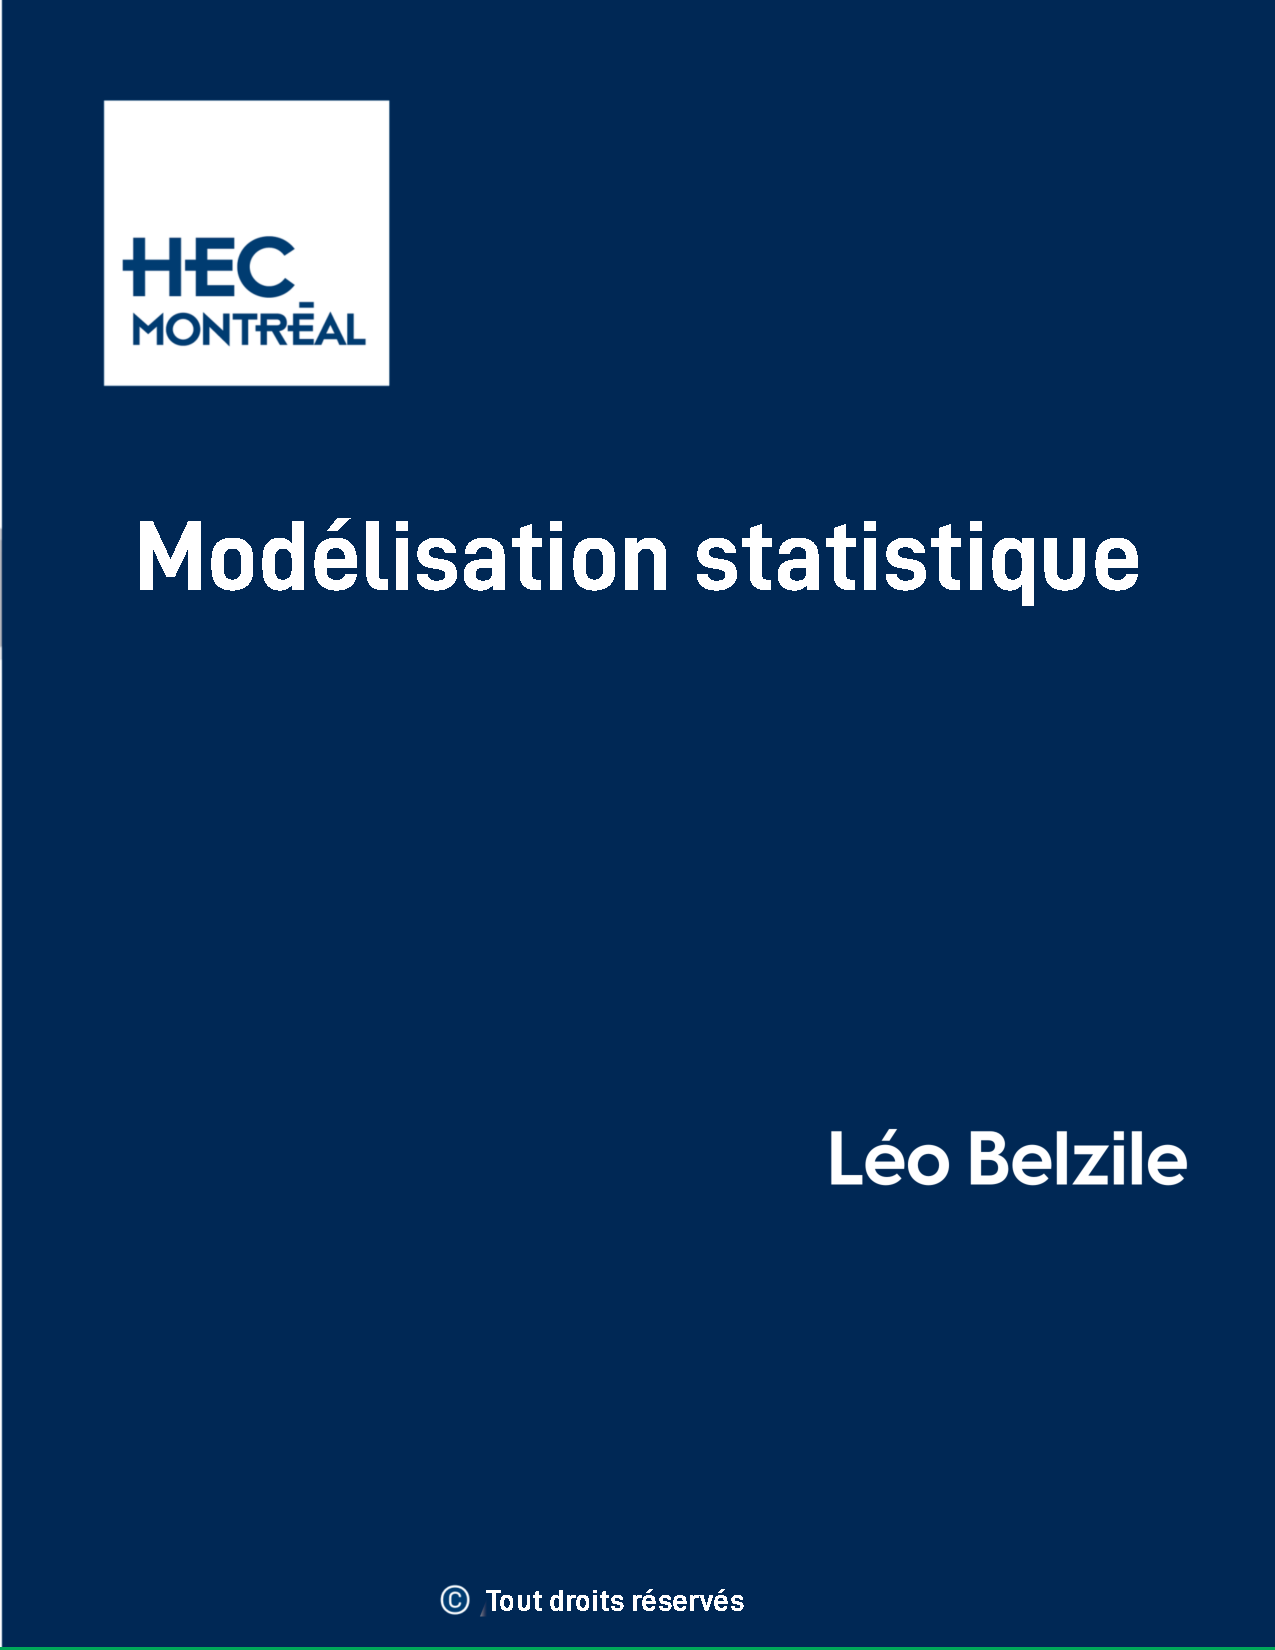
\includepdf{images/pagedecouverture.pdf}

\renewcommand*\contentsname{Table des matières}
{
\setcounter{tocdepth}{2}
\tableofcontents
}

\mainmatter
\bookmarksetup{startatroot}

\chapter*{Bienvenue}\label{bienvenue}
\addcontentsline{toc}{chapter}{Bienvenue}

\markboth{Bienvenue}{Bienvenue}

Ces notes sont l'oeuvre de Léo Belzile (HEC Montréal) et sont mises à
disposition sous la
\href{https://creativecommons.org/licenses/by-nc-sa/4.0/legalcode.fr}{Licence
publique Creative Commons Attribution - Utilisation non commerciale -
Partage dans les mêmes conditions 4.0 International}.

Ce cours traite de modélisation des données. Une citation célèbre
attribuée à George Box dit que

\begin{quote}
tous les modèles sont faux, mais certains sont utiles.
\end{quote}

Ce point de vue est réducteur; McCullagh et Nelder
(\citeproc{ref-McCullagh.Nelder:1989}{1989}) (traduction libre)
expliquent dans le préambule de leur livre

\begin{quote}
La modélisation en science demeure, du moins partiellement, un art.
Certains principes existent, en revanche, pour guider le modélisateur.
Le premier est que tous les modèles sont faux; mais que \textbf{certains
sont meilleurs} et \textbf{le modélisateur doit chercher le meilleur à
sa portée}. En même temps, il est sage de reconnaître que la quête
perpétuelle de la vérité n'est pas envisageable.
\end{quote}

Et David R. Cox (traduction libre), de rajouter

\begin{quote}
\ldots il n'est pas utile de simplement énoncer que tout modèle est
faux. L'idée même de modèle sous-tend une notion de simplification et
d'idéalisation. L'idée qu'un système physique, biologique ou
sociologique complexe puisse être décrit de manière exacte par quelques
formules est franchement absurde. La construction de
\textbf{représentations idéalisées qui capturent les aspects stables les
plus importants du système} est néanmoins une partie essentielle de
toute analyse scientifique et les modèles statistiques ne diffèrent pas
en cela d'autres types de modèles.
\end{quote}

Pourquoi utiliser des modèles?
\href{https://krugman.blogs.nytimes.com/2010/11/18/debt-deleveraging-and-the-liquidity-trap/}{Paul
Krugman écrivait en 2010 dans son blogue}

\begin{quote}
La réponse que je donnerais est que les modèles sont un outil énormément
important pour clarifier ses pensées. Vous n'avez pas à avoir une foi
aveugle en votre modèle {[}\ldots{]} pour croire qu'en mettant sur pied
une description simplifiée, mais complète du fonctionnement du système
{[}\ldots{]} vous permet de gagner une compréhension plus sophistiquée
de la situation réelle. Les personnes qui n'utilisent pas de modèles
finissent par se baser sur des slogans beaucoup plus simplistes que les
modèles.
\end{quote}

\section*{Contenu du cours}\label{contenu-du-cours}
\addcontentsline{toc}{section}{Contenu du cours}

\markright{Contenu du cours}

L'inférence statistique a pour but de tirer des conclusions formelles à
partir de données. Dans le cadre de la recherche scientifique, le
chercheur formule une hypothèse, collecte des données et conclut quant à
la plausibilité de son hypothèse.

On distingue deux types de jeux de données: les données
\textbf{expérimentales} sont typiquement collectées en milieu contrôlé
suivant un protocole d'enquête et un plan d'expérience: elles servent à
répondre à une question prédéterminée. L'approche expérimentale est
désirable pour éviter le «jardin des embranchements» (une
\href{http://www.stat.columbia.edu/~gelman/research/unpublished/p_hacking.pdf}{allégorie
signifiant qu'un chercheur peut raffiner son hypothèse à la lumière des
données, sans ajustement pour des variables confondantes}), mais elle
n'est pas toujours réalisable: par exemple, un économiste ne peut pas
modifier les taux d'intérêts pour observer les impacts sur le taux
d'épargne des consommateurs. Lorsque les données ont été collectées
préalablement à d'autres fins, on parle de données
\textbf{observationnelles}.

Par modèle, on entendra la spécification d'une loi aléatoire pour les
données et une équation reliant les paramètres ou l'espérance
conditionnelle d'une variable réponse \(Y\) à un ensemble de variables
explicatives \(\mathbf{X}\). Ce modèle peut servir à des fins de
prédiction (modèle prédictif) ou pour tester des hypothèses de recherche
concernant les effets de ces variables (modèle explicatif). Ces deux
objectifs ne sont pas mutuellement exclusifs même si on fait parfois une
distinction entre inférence et prédiction.

Un modèle prédictif permet d'obtenir des prédictions de la valeur de
\(Y\) pour d'autres combinaisons de variables explicatives ou des
données futures. Par exemple, on peut chercher à prédire la consommation
énergétique d'une maison en fonction de la météo, du nombre d'habitants
de la maison et de sa taille. La plupart des boîtes noires utilisées en
apprentissage automatique tombent dans la catégorie des modèles
prédictifs: ces modèles ne sont pas interprétables et ignorent parfois
la structure inhérente aux données.

Par contraste, les modèles explicatifs sont souvent simples et
interprétables, et les modèles de régressions sont fréquemment utilisés
pour l'inférence. On se concentrera dans ce cours sur les modèles
explicatifs. Par exemple, on peut chercher à déterminer

\begin{itemize}
\tightlist
\item
  Est-ce que les décisions intégrées (décision combinée d'achat et de
  quantité) sont préférables aux décisions séquentielles (décision
  d'acheter, puis choix de la quantité) lors de l'achat d'un produit en
  ligne (\citeproc{ref-Duke.Amir:2023}{Duke et Amir 2023})?
\item
  Qu'est-ce qui est le plus distrayant pour les utilisateurs de la
  route: parler au cellulaire, texter en conduisant, consulter sa montre
  intelligente (\citeproc{ref-Brodeur:2021}{Brodeur et al. 2021})?
\item
  Quel est l'impact de de l'inadéquation entre l'image d'un produit et
  sa description (\citeproc{ref-Lee.Choi:2019}{Lee et Choi 2019})?
\item
  Qu'est-ce qui explique que les prix de l'essence soient plus élevés en
  Gaspésie qu'ailleurs au Québec?
  \href{https://ici.radio-canada.ca/nouvelle/1463520/prix-essence-gaspesie-rapport-regie-energie}{Un
  rapport de surveillance des prix de l'essence en Gaspésie par la Régie
  de l'énergie se penche sur la question.}
\item
  Est-ce que les examens pratiques de conduite en Grande-Bretagne sont
  plus faciles dans les régions à faible densité de population?
  \href{https://www.theguardian.com/world/2019/aug/23/an-easy-ride-scottish-village-fuels-debate-driving-test-pass-rates}{Une
  analyse du journal britannique \emph{The Guardian}} laisse penser que
  c'est le cas.
\item
  Quelle est la perception environnementale d'un emballage de carton
  (versus de plastique) s'il englobe un contenant en plastique
  (\citeproc{ref-Sokolova:2023}{Sokolova, Krishna, et Döring 2023}).
\item
  Quel est l'impact psychologique des suggestions sur le montant de dons
  (\citeproc{ref-Moon.VanEpps:2023}{Moon et VanEpps 2023})?
\item
  Est-ce que la visioconférence réduit le nombre d'interactions et
  d'idée créatives générées lors d'une réunion, par rapport à une
  rencontre en personne (\citeproc{ref-Brucks.Levav:2022}{Brucks et
  Levav 2022})?
\end{itemize}

\bookmarksetup{startatroot}

\chapter{Introduction}\label{intro}

Ce chapitre couvre des rappels mathématiques de probabilité et
statistique d'ordinaire couverts dans un cours de niveau collégial ou
préuniversitaire.

\section{Population et échantillons}\label{population-echantillon}

Ce qui différencie la statistique des autres sciences est la prise en
compte de l'incertitude et de la notion d'aléatoire. Règle générale, on
cherche à estimer une caractéristique d'une population définie à l'aide
d'un échantillon (un sous-groupe de la population) de taille restreinte.

La \textbf{population d'intérêt} est un ensemble d'individus formant la
matière première d'une étude statistique. Par exemple, pour l'Enquête
sur la population active (EPA) de Statistique Canada, « la population
cible comprend la population canadienne civile non institutionnalisée de
15 ans et plus ». Même si on faisait un recensement et qu'on
interrogeait tous les membres de la population cible, la caractéristique
d'intérêt peut varier selon le moment de la collecte; une personne peut
trouver un emploi, quitter le marché du travail ou encore se retrouver
au chômage. Cela explique la variabilité intrinsèque.

En général, on se base sur un \textbf{échantillon} pour obtenir de
l'information parce que l'acquisition de données est coûteuse.
L'\textbf{inférence statistique} vise à tirer des conclusions, pour
toute la population, en utilisant seulement l'information contenue dans
l'échantillon et en tenant compte des sources de variabilité. Le sondeur
George Gallup (traduction libre) a fait cette merveilleuse analogie
entre échantillon et population:

\begin{quote}
«Il n'est pas nécessaire de manger un bol complet de soupe pour savoir
si elle est trop salé; pour autant qu'elle ait été bien brassée, une
cuillère suffit.»
\end{quote}

Un \textbf{échantillon} est un sous-groupe d'individus de la population.
Si on veut que ce dernier soit représentatif, il devrait être tiré
aléatoirement de la population, ce qui nécessite une certaine
connaissance de cette dernière. Au siècle dernier, les bottins
téléphoniques pouvaient servir à créer des plans d'enquête. C'est un
sujet complexe et des cours entiers d'échantillonnage y sont consacrés.
Même si on ne collectera pas de données, il convient de noter la
condition essentielle pour pouvoir tirer des conclusions fiables à
partir d'un échantillon: ce dernier doit être représentatif de la
population étudiée, en ce sens que sa composition doit être similaire à
celle de la population, et aléatoire. On doit ainsi éviter les biais de
sélection, notamment les échantillons de commodité qui consistent en une
sélection d'amis et de connaissances.

Si notre échantillon est \textbf{aléatoire}, notre mesure d'une
caractéristique d'intérêt le sera également et la conclusion de notre
procédure de test variera d'un échantillon à l'autre. Plus la taille de
ce dernier est grande, plus on obtiendra une mesure précise de la
quantité d'intérêt. L'exemple suivant illustre pourquoi le choix de
l'échantillon est important.

\begin{example}[Gallup et l'élection présidentielle américaine de
1936]\protect\hypertarget{exm-Gallup}{}\label{exm-Gallup}

Désireuse de prédire le résultat de l'élection présidentielle américaine
de 1936, la revue \emph{Literary Digest} a sondé 10 millions d'électeurs
par la poste, dont 2.4 millions ont répondu au sondage en donnant une
nette avance au candidat républicain Alf Landon (57\%) face au président
sortant Franklin D. Roosevelt (43\%). Ce dernier a néanmoins remporté
l'élection avec 62\% des suffrages, une erreur de prédiction de 19\%. Le
plan d'échantillonnage avait été conçu en utilisant des bottins
téléphoniques, des enregistrements d'automobiles et des listes de
membres de clubs privés, etc.:
\href{https://www.jstor.org/stable/2749114}{la non-réponse
différentielle et un échantillon biaisé} vers les classes supérieures
sont en grande partie responsable de cette erreur.

Gallup avait de son côté correctement prédit la victoire de Roosevelt en
utilisant un échantillon aléatoire de (seulement) 50 000 électeurs. Vous
pouvez lire
l'\href{https://ozanozbey.medium.com/two-lessons-of-sampling-bias-from-1936-us-election-e4e96bd42be}{histoire
complète (en anglais)}.

\end{example}

\section{Types de variables}\label{types-de-variables}

Le résultat d'une collecte de données est un tableau, ou base de
données, contenant sur chaque ligne des observations et en colonne des
variables. Le Tableau~\ref{tbl-data-renfe} donne un exemple de
structure.

\begin{itemize}
\tightlist
\item
  Une \textbf{variable} représente une caractéristique de la population
  d'intérêt, par exemple le sexe d'un individu, le prix d'un article,
  etc.
\item
  une \textbf{observation}, parfois appelée donnée, est un ensemble de
  mesures collectées sous des conditions identiques, par exemple pour un
  individu ou à un instant donné.
\end{itemize}

\begin{longtable}[]{@{}rllllrl@{}}

\caption{\label{tbl-data-renfe}Premières lignes de la base de données
\texttt{renfe}, qui contient les prix de 10K billets de train entre
Barcelone et Madrid. Les colonnes \texttt{prix} et \texttt{duree} sont
des variables numériques continues, les autres des variables
catégorielles.}

\tabularnewline

\toprule\noalign{}
prix & type & classe & tarif & dest & duree & jour \\
\midrule\noalign{}
\endhead
\bottomrule\noalign{}
\endlastfoot
143.4 & AVE & Preferente & Promo & Barcelone-Madrid & 190 & 6 \\
181.5 & AVE & Preferente & Flexible & Barcelone-Madrid & 190 & 2 \\
86.8 & AVE & Preferente & Promo & Barcelone-Madrid & 165 & 7 \\
86.8 & AVE & Preferente & Promo & Barcelone-Madrid & 190 & 7 \\
69.0 & AVE-TGV & Preferente & Promo & Barcelone-Madrid & 175 & 4 \\

\end{longtable}

Le choix de modèle statistique ou de test dépend souvent du type de
variables collectées. Les variables peuvent être de plusieurs types:
quantitatives (discrètes ou continues) si elles prennent des valeurs
numériques, qualitatives (binaires, nominales ou ordinales) si elles
peuvent être décrites par un adjectif; je préfère le terme catégorielle,
plus évocateur.

La plupart des modèles avec lesquels nous interagirons sont des modèles
dits de régression, dans lesquelles on modélisation la moyenne d'une
variable quantitative en fonction d'autres variables dites explicatives.
Il y a deux types de variables numériques:

\begin{itemize}
\tightlist
\item
  une variable discrète prend un nombre dénombrable de valeurs; ce sont
  souvent des variables de dénombrement ou des variables dichotomiques.
\item
  une variable continue peut prendre (en théorie) une infinité de
  valeurs, même si les valeurs mesurées sont arrondies ou mesurées avec
  une précision limitée (temps, taille, masse, vitesse, salaire). Dans
  bien des cas, nous pouvons considérer comme continues des variables
  discrètes si elles prennent un assez grand nombre de valeurs.
\end{itemize}

Les variables catégorielles représentent un ensemble fini de
possibilités. On les regroupe en deux types, pour lesquels on ne fera
pas de distinction:

\begin{itemize}
\tightlist
\item
  nominales s'il n'y a pas d'ordre entre les modalités (sexe, couleur,
  pays d'origine) ou
\item
  ordinale (échelle de Likert, tranche salariale).
\end{itemize}

La codification des modalités des variables catégorielle est arbitraire;
en revanche, on préservera l'ordre lorsqu'on représentera graphiquement
les variables ordinales. Lors de l'estimation, chaque variable
catégorielle doit est transformée en un ensemble d'indicateurs binaires
0/1: il est donc essentiel de déclarer ces dernières dans votre logiciel
statistique, surtout si elles sont parfois encodées dans la base de
données à l'aide de valeurs entières.

\section{Variables aléatoires}\label{variable-aleatoire}

Suppsons qu'on cherche à décrire le comportement d'un phénomène
aléatoire. Pour ce faire, on cherche à décrire l'ensemble des valeurs
possibles et leur probabilité/fréquence relative au sein de la
population: ces dernières sont encodées dans la loi de la variable
aléatoire.

On dénote les variables aléatoires par des lettres majuscules, et leurs
réalisations par des minuscules: par exemple,
\(Y \sim \mathsf{normale}(\mu, \sigma^2)\) indique que \(Y\) suit une
loi normale de paramètres \(\mu \in \mathbb{R}\) et \(\sigma > 0\). On
parle de famille de lois si la valeur des paramètres ne sont pas
spécifiées; si on fixe plutôt ces dernière, on obtient une
représentation qui encode les probabilité.

\begin{definition}[Fonctions de répartition, de masse et de
densité]\protect\hypertarget{def-repartition}{}\label{def-repartition}

La \textbf{fonction de répartition} \(F(y)\) donne la probabilité
cumulative qu'un événement n'excède pas une variable donnée,
\(F(y) = \mathsf{Pr}(Y \leq y)\). Si la variable \(Y\) prend des valeurs
discrètes, alors on utilise la \textbf{fonction de masse}
\(f(y)=\mathsf{Pr}(Y=y)\) qui donne la probabilité pour chacune des
valeurs de \(y\). Si la variable \(Y\) est continue, aucune valeur
numérique de \(y\) n'a de probabilité non-nulle et \(\Pr(Y=y) = 0\) pour
toute valeur réelle \(y\); la \textbf{densité}, aussi dénotée \(f(x)\),
est une fonction est non-négative et satisfait
\(\int_{\mathbb{R}} f(x) \mathrm{d}x=1\): elle décrit la probabilité
d'obtenir un résultat dans un ensemble donné des réels \(\mathbb{R}\),
pour n'importe lequel intervalle. La densité sert à estimer la
probabilité que la variable continue \(Y\) appartienne à un ensemble
\(B\), via \(\mathsf{Pr}(Y \in B) = \int_B f(y) \mathrm{d} y\); la
fonction de répartition est ainsi définie comme
\(F(y) = \int_{-\infty}^y f(x) \mathrm{d} x\).

\begin{figure}[ht!]

\centering{

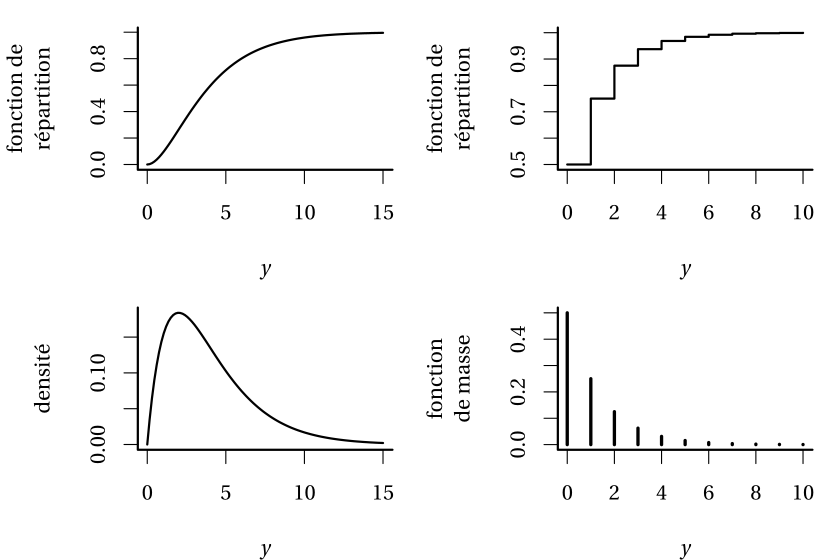
\includegraphics[width=0.85\textwidth,height=\textheight]{images/02-ttest-DF_illustration_fr.png}

}

\caption{\label{fig-distributions}Fonctions de répartition (panneau
supérieur) et fonctions de densité et de masse (panneau inférieur) pour
une loi continue (gauche) et discrète (droite).}

\end{figure}%

\end{definition}

Un premier cours de statistique débute souvent par la présentation de
statistiques descriptives comme la moyenne et l'écart-type. Ce sont des
estimateurs des moments (centrés), qui caractérisent la loi du phénomène
d'intérêt. Dans le cas de la loi normale unidimensionnelle, qui a deux
paramètres, l'espérance et la variance caractérisent complètement le
modèle.

\begin{definition}[Moments]\protect\hypertarget{def-moments}{}\label{def-moments}

Soit \(Y\) une variable aléatoire de fonction de densité (ou de masse)
\(f(x)\). On définit l'espérance d'une variable aléatoire \(Y\) comme
\begin{align*}
\mathsf{E}(Y)=\int_{\mathbb{R}} y f(y) \mathrm{d} y.
\end{align*} L'espérance est la « moyenne théorique», ou moment de
premier ordre : dans le cas discret,
\(\mu = \mathsf{E}(Y)=\sum_{y \in \mathcal{y}} y \mathsf{Pr}(y=y)\), où
\(\mathcal{Y}\) représente le support de la loi, à savoir les valeurs
qui peuvent prendre \(Y\). Plus généralement, l'espérance d'une fonction
\(g(y)\) pour une variable aléatoire \(Y\) est simplement l'intégrale de
\(g(y)\) pondérée par la densité \(f(y)\). De même, si l'intégrale est
convergente, la \textbf{variance} est \begin{align*}
\mathsf{Va}(Y)&=\int_{\mathbb{R}} (y-\mu)^2 f(y) \mathrm{d} y \\&=\mathsf{E}\{Y-\mathsf{E}(Y)\}^2 \\&= \mathsf{E}(Y^2) - \{\mathsf{E}(Y)\}^2.
\end{align*}

L'écart-type est défini comme la racine carrée de la variance,
\(\mathsf{sd}(Y)=\sqrt{\mathsf{Va}(Y)}\): elle est exprimé dans les
mêmes unités que celle de \(Y\) et donc plus facilement interprétable.

La notion de moments peut être généralisé à des vecteurs. Si
\(\boldsymbol{Y}\) est un \(n\)-vecteur, comprenant par exemple dans le
cadre d'une régression des mesures d'un ensemble d'observations, alors
l'espérance est calculée composante par composante,

\begin{align*}
\mathsf{E}(\boldsymbol{Y}) &= \boldsymbol{\mu}=
\begin{pmatrix}
\mathsf{E}(Y_1) &
\cdots  &
\mathsf{E}(Y_n)
\end{pmatrix}^\top
\end{align*} tandis que la matrice \(n \times n\) de deuxième moments
centrés de \(\boldsymbol{Y}\), dite matrice de variance ou matrice de
\textbf{covariance}, est \begin{align*}
\mathsf{Va}(\boldsymbol{Y}) &= \boldsymbol{\Sigma} = \begin{pmatrix} \mathsf{Va}(Y_1) & \mathsf{Co}(Y_1, Y_2)  & \cdots & \mathsf{Co}(Y_1, Y_n) \\
\mathsf{Co}(Y_2, Y_1) & \mathsf{Va}(Y_2) & \ddots & \vdots \\
\vdots & \ddots & \ddots & \vdots \\
\mathsf{Co}(Y_n, Y_1) & \mathsf{Co}(Y_n, Y_2) &\cdots & \mathsf{Va}(Y_n)
\end{pmatrix}
\end{align*} Le \(i\)e élément diagonal de \(\boldsymbol{\Sigma}\),
\(\sigma_{ii}=\sigma_i^2\), est la variance de \(Y_i\), tandis que les
éléments hors de la diagonale, \(\sigma_{ij}=\sigma_{ji}\)
\((i \neq j)\), sont les covariances des paires \begin{align*}
\mathsf{Co}(Y_i, Y_j) = \int_{\mathbb{R}^2} (y_i-\mu_i)(y_j-\mu_j) f_{Y_i, Y_j}(y_i, y_j) \mathrm{d} y_i \mathrm{d} y_j.
\end{align*} Par construction, la matrice de covariance
\(\boldsymbol{\Sigma}\) est symmétrique. Il est d'usage de considérer la
relation deux-à-deux de variables standardisées, afin de séparer la
dépendance linéaire de la variabilité de chaque composante. La
\textbf{corrélation linéaire} entre \(Y_i\) et \(Y_j\) est
\begin{align*}
\rho_{ij}=\mathsf{Cor}(Y_i,Y_j)=\frac{\mathsf{Co}(Y_i, Y_j)}{\sqrt{\mathsf{Va}(Y_i)}\sqrt{\mathsf{Va}(Y_j)}}=\frac{\sigma_{ij}}{\sigma_i\sigma_j}.
\end{align*} La matrice de corrélation de \(\boldsymbol{Y}\) est une
matrice symmétrique \(n\times n\) avec des uns sur la diagonale et les
corrélations des pairs hors diagonale, \begin{align*}
\mathsf{Cor}(\boldsymbol{Y})=
\begin{pmatrix}
1 & \rho_{12} & \rho_{13} & \cdots & \rho_{1n}\\
\rho_{21} & 1 & \rho_{23} & \cdots & \rho_{2n} \\
\rho_{31} & \rho_{32} & 1 & \ddots & \rho_{3n} \\
\vdots & \vdots & \ddots & \ddots & \vdots \\
\rho_{n1} & \rho_{n2} & \rho_{n3} & \cdots & 1
\end{pmatrix}.
\end{align*} Nous modéliserons la matrice de covariance ou de
corrélation des données corrélées et longitudinales par individus du
même groupe (ou du même individu pour les mesures répétées) dans le
\href{donnees-longitudinales-correlees}{Chapitre 5}.

\end{definition}

\begin{definition}[Biais]\protect\hypertarget{def-biais}{}\label{def-biais}

Le biais d'un estimateur \(\hat{\theta}\) pour un paramètre \(\theta\)
est \begin{align*}
\mathsf{biais}(\hat{\theta})=\mathsf{E}(\hat{\theta})- \theta
\end{align*} L'estimateur est non biaisé si
\(\mathsf{biais}(\hat{\theta})=0\).

\end{definition}

\begin{example}[Estimateurs sans
biais]\protect\hypertarget{exm-estimateurs-non-biaises}{}\label{exm-estimateurs-non-biaises}

L'estimateur sans biais de l'espérance de \(Y\) pour un échantillon
aléatoire simple \(Y_1, \ldots, Y_n\) est la moyenne empirique
\(\overline{Y}_n = n^{-1} \sum_{i=1}^n Y_i\) et celui de la variance
\(S_n = (n-1)^{-1} \sum_{i=1}^n (Y_i-\overline{Y})^2\).

\end{example}

Un estimateur sans biais est souhaitable, mais pas toujours optimal.
Quelquefois, il n'existe pas d'estimateur non-biaisé pour un paramètre!
Dans plusieurs cas, on cherche un estimateur qui minimise l'erreur
quadratique moyenne.

Souvent, on cherche à balancer le biais et la variance: rappelez-vous
qu'un estimateur est une variable aléatoire (étant une fonction de
variables aléatoires) et qu'il est lui-même variable: même s'il est sans
biais, la valeur numérique obtenue fluctuera d'un échantillon à l'autre.

\begin{definition}[Erreur quadratique
moyenne]\protect\hypertarget{def-eqm}{}\label{def-eqm}

On peut chercher un estimateur qui minimise l'erreur quadratique
moyenne, \begin{align*}
\mathsf{EQM}(\hat{\theta}) = \mathsf{E}\{(\hat{\theta}-\theta)^2\}=\mathsf{Va}(\hat{\theta}) + \{\mathsf{E}(\hat{\theta})\}^2.
\end{align*} Cette fonction objective est donc un compromis entre le
carré du biais et la variance de l'estimateur.

\end{definition}

La plupart des estimateurs que nous considérerons dans le cadre du cours
sont des estimateurs du maximum de vraisemblance. Ces derniers sont
asymptotiquement efficaces, c'est-à-dire qu'ils minimisent l'erreur
quadratique moyenne parmi tous les estimateurs possibles quand la taille
de l'échantillon est suffisamment grande. Ils ont également d'autre
propriétés qui les rendent attractifs comme choix par défaut pour
l'estimation. Il ne sont pas nécessairement sans biais

\section{Loi discrètes}\label{loi-discruxe8tes}

Plusieurs lois aléatoires décrivent des phénomènes physiques simples et
ont donc une justification empirique; on revisite les distributions ou
loi discrètes les plus fréquemment couvertes.

\begin{definition}[Loi de
Bernoulli]\protect\hypertarget{def-loibern}{}\label{def-loibern}

On considère un phénomène binaire, comme le lancer d'une pièce de
monnaie (pile/face). De manière générale, on associe les deux
possibilités à succès/échec et on suppose que la probabilité de
``succès'' est \(p\). Par convention, on représente les échecs (non) par
des zéros et les réussites (oui) par des uns. Donc, si la variable \(Y\)
vaut \(0\) ou \(1\), alors \(\mathsf{Pr}(Y=1)=p\) et la probabilité
complémentaire est \(\mathsf{Pr}(Y=0)=1-p\). La fonction de masse de la
\href{https://fr.wikipedia.org/wiki/Loi_de_Bernoulli}{loi Bernoulli}
s'écrit de façon plus compacte \begin{align*}
\mathsf{Pr}(Y=y) = p^y (1-p)^{1-y}, \quad y=0, 1.
\end{align*}

\end{definition}

Un calcul rapide montre que \(\mathsf{E}(Y)=p\) et
\(\mathsf{Va}(Y)=p(1-p)\). Effectivement, \begin{align*}
\mathsf{E}(Y) = \mathsf{E}(Y^2) = p \cdot 1 + (1-p) \cdot 0 = p.
\end{align*}

Voici quelques exemples de questions de recherches comprenant une
variable réponse binaire:

\begin{itemize}
\tightlist
\item
  est-ce qu'un client potentiel a répondu favorablement à une offre
  promotionnelle?
\item
  est-ce qu'un client est satisfait du service après-vente?
\item
  est-ce qu'une firme va faire faillite au cours des trois prochaines
  années?
\item
  est-ce qu'un participant à une étude réussit une tâche assignée?
\end{itemize}

Plus généralement, on aura accès à des données aggrégées.

\begin{example}[Loi
binomiale]\protect\hypertarget{exm-loibinom}{}\label{exm-loibinom}

Si les données représentent la somme d'événements Bernoulli
indépendants, la loi du nombre de réussites \(Y\) pour un nombre
d'essais donné \(m\) est dite
\href{https://fr.wikipedia.org/wiki/Loi_binomiale}{binomiale}, dénotée
\(\mathsf{Bin}(m, p)\); sa fonction de masse est \begin{align*}
\mathsf{Pr}(Y=y) = \binom{m}{y}p^y (1-p)^{1-y}, \quad y=0, 1.
\end{align*} La vraisemblance pour un échantillon de la loi binomiale
est (à constante de normalisation près qui ne dépend pas de \(p\)) la
même que pour un échantillon aléatoire de \(m\) variables Bernoulli
indépendantes. L'espérance d'une variable binomiale est
\(\mathsf{E}(Y)=mp\) et la variance \(\mathsf{Va}(Y)=mp(1-p)\).

\end{example}

On peut ainsi considérer le nombre de personnes qui ont obtenu leur
permis de conduire parmi \(m\) candidat(e)s ou le nombre de clients sur
\(m\) qui ont passé une commande de plus de 10\$ dans un magasin.

Plus généralement, on peut considérer des variables de dénombrement qui
prennent des valeurs entières. Parmi les exemples de questions de
recherches comprenant une variable réponse de dénombrement:

\begin{itemize}
\tightlist
\item
  le nombre de réclamations faites par un client d'une compagnie
  d'assurance au cours d'une année.
\item
  le nombre d'achats effectués par un client depuis un mois.
\item
  le nombre de tâches réussies par un participant lors d'une étude.
\end{itemize}

La densité d'une loi Student standard avec \(\nu\) degrés de liberté est
\begin{align*}
f(y; \nu) = \frac{\Gamma \left( \frac{\nu+1}{2}\right)}{\Gamma\left(\frac{\nu}{2}\right)
\sqrt{\nu\pi}}\left(1+\frac{y^{2}}{\nu}\right)^{-\frac{\nu+1}{2}}.
\end{align*} La loi a des ailes à décroissance polynomiale, est
symmétrique autour de zéro et unimodale. Quand \(\nu \to \infty\), on
recouvre une loi normale, mais les ailes sont plus lourdes que la loi
normale. Effectivement, seuls les \(\nu-1\) premiers moments de la
distribution existent: la loi \(\mathsf{Student}(2)\) n'a pas de
variance.

Si les \(n\) observations indépendantes et identiquement distribuées
\(Y_i \sim \mathsf{normale}(\mu, \sigma^2)\), alors la moyenne empirique
centrée, divisée par la variance empirique, \((\overline{Y}-\mu)/S^2\),
suit une loi Student-\(t\) avec \(n-1\) degrés de liberté.

\begin{figure}[ht!]

\centering{

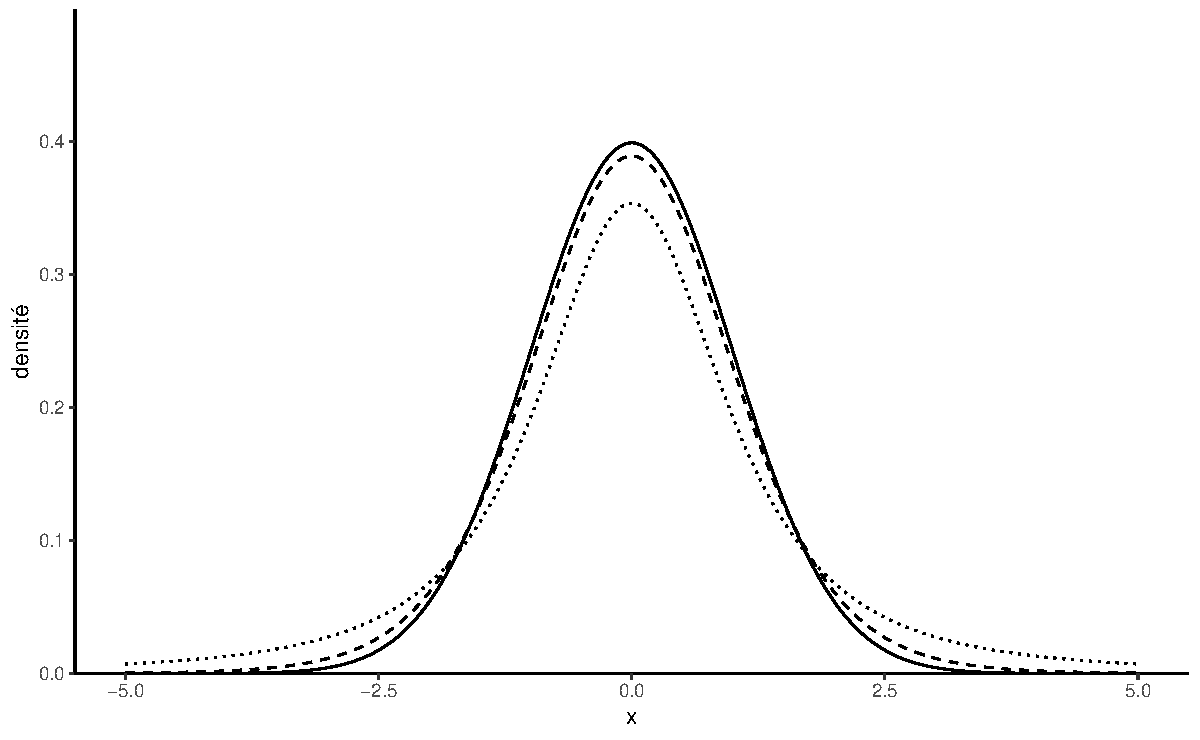
\includegraphics[width=0.5\textwidth,height=\textheight]{introduction_files/figure-pdf/fig-densite-Student-1.pdf}

}

\caption{\label{fig-densite-Student}Comparaison de la densité
Student-\(t\) versus normale pour différents degrés de liberté avec
\(\nu=2\) (pointillé), \(\nu=10\) (traitillé) et la loi normale
(\(\nu = \infty)\).}

\end{figure}%

:::

\begin{definition}[Loi de
Fisher]\protect\hypertarget{def-loiF}{}\label{def-loiF}

La loi de Fisher, ou loi \(F\), sert à déterminer le comportement en
grand échantillon de statistiques de test pour la comparaison de
plusieurs moyennes (analyse de variance) sous un postulat de normalité
des observations.

La loi \(F\), dite de Fisher et dénotée
\(\mathsf{Fisher}(\nu_1, \nu_2)\), est obtenue en divisant deux
variables khi-deux indépendantes de degrés de liberté \(\nu_1\) et
\(\nu_2\). Spécifiquement, si \(Y_1 \sim \chi^2_{\nu_1}\) et
\(Y_2 \sim \chi^2_{\nu_2}\), alors \begin{align*}
F = \frac{Y_1/\nu_1}{Y_2/\nu_2} \sim \mathsf{Fisher}(\nu_1, \nu_2)
\end{align*}

La loi de Fisher tend vers une loi \(\chi^2_{\nu_1}\) quand
\(\nu_2 \to \infty\).

\end{definition}

\section{Graphiques}\label{graphiques}

Cette section sert à réviser les principales représentations graphiques
de jeux de données selon la catégorie des variables.

Le principal type de graphique pour représenter la distribution d'une
variable catégorielle est le diagramme en bâtons, dans lequel la
fréquence de chaque catégorie est présentée sur l'axe des ordonnées
(\(y\)) en fonction de la modalité, sur l'axe des abscisses (\(x\)), et
ordonnées pour des variables ordinales. Cette représentation est en tout
point supérieur au
\href{http://www.perceptualedge.com/articles/08-21-07.pdf}{diagramme en
camembert}, une engeance répandu qui devrait être honnie (notamment
parce que l'humain juge mal les différences d'aires, qu'une simple
rotation change la perception du graphique et qu'il est difficile de
mesurer les proportions) --- ce n'est pas de la tarte!

\begin{figure}[ht!]

\centering{

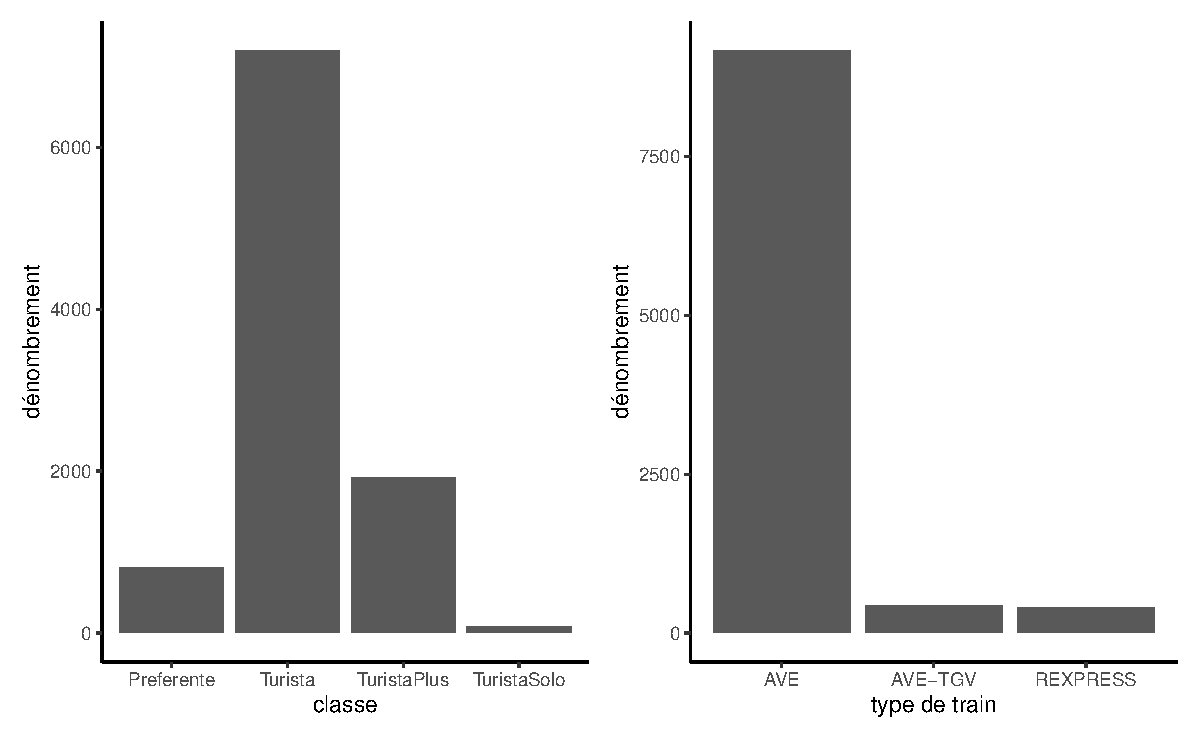
\includegraphics[width=0.85\textwidth,height=\textheight]{introduction_files/figure-pdf/fig-barplotrenfe-1.pdf}

}

\caption{\label{fig-barplotrenfe}Diagramme en bâtons pour la classe des
billets de trains du jeu de données Renfe.}

\end{figure}%

Puisque les variables continues peuvent prendre autant de valeurs
distinctes qu'il y a d'observations, on ne peut simplement compter le
nombre d'occurrence par valeur unique. On regroupera plutôt dans un
certain nombre d'intervalle, en discrétisant l'ensemble des valeurs en
classes pour obtenir un histogramme. Le nombre de classes dépendra du
nombre d'observations si on veut que l'estimation ne soit pas impactée
par le faible nombre d'observations par classe: règle générale, le
nombre de classes ne devrait pas dépasser \(\sqrt{n}\), où \(n\) est le
nombre d'observations de l'échantillon. On obtiendra la fréquence de
chaque classe, mais si on normalise l'histogramme (de façon à ce que
l'aire sous les bandes verticales égale un), on obtient une
approximation discrète de la fonction de densité. Faire varier le nombre
de classes permet parfois de faire apparaître des caractéristiques de la
variable (notamment la multimodalité, l'asymmétrie et les arrondis).

Puisque qu'on groupe les observations en classe pour tracer
l'histogramme, il est difficile de voir l'étendue des valeurs que prenne
la variable: on peut rajouter des traits sous l'histogramme pour
représenter les valeurs uniques prises par la variable, tandis que la
hauteur de l'histogramme nous renseigne sur leur fréquence relative.

\begin{figure}[ht!]

\centering{

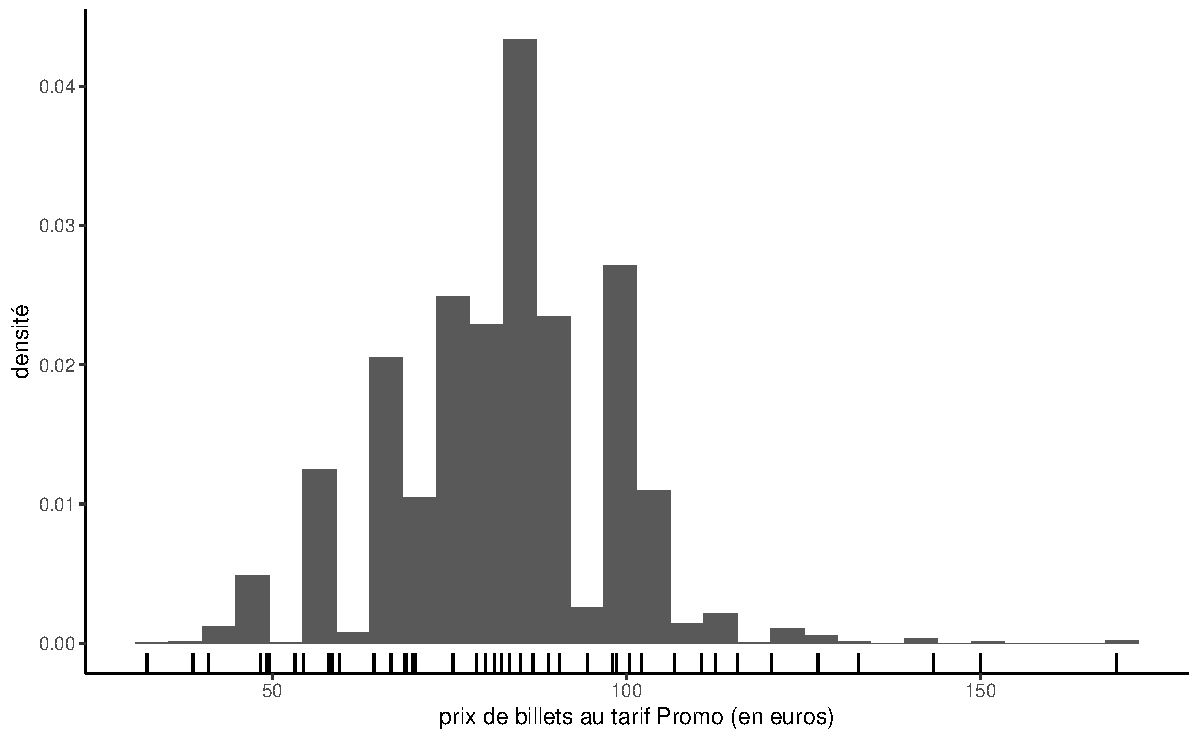
\includegraphics[width=0.85\textwidth,height=\textheight]{introduction_files/figure-pdf/fig-histrenfe-1.pdf}

}

\caption{\label{fig-histrenfe}Histogramme du prix des billets au tarif
Promo de trains du jeu de données Renfe}

\end{figure}%

\begin{definition}[Boîte à
moustaches]\protect\hypertarget{def-boxplot}{}\label{def-boxplot}

Elle représente graphiquement cinq statistiques descriptives.

\begin{itemize}
\tightlist
\item
  La boîte donne les 1e, 2e et 3e quartiles \(q_1, q_2, q_3\). Il y a
  donc 50\% des observations sont au-dessus/en-dessous de la médiane
  \(q_2\) qui sépare en deux la boîte.
\item
  La longueur des moustaches est moins de \(1.5\) fois l'écart
  interquartile \(q_3-q_1\) (tracée entre 3e quartile et le dernier
  point plus petit que \(q_3+1.5(q_3-q_1)\), etc.)
\item
  Les observations au-delà des moustaches sont encerclées. Notez que
  plus le nombre d'observations est élevé, plus le nombres de valeurs
  aberrantes augmente. C'est un défaut de la boîte à moustache, qui a
  été conçue pour des jeux de données qui passeraient pour petits selon
  les standards actuels.
\end{itemize}

\begin{figure}[ht!]

{\centering 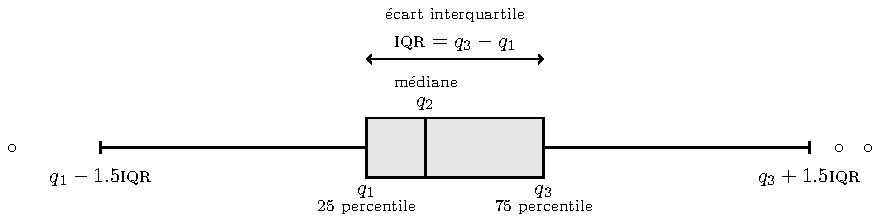
\includegraphics[width=0.85\textwidth,height=\textheight]{images/01-intro-boiteamoustache.pdf}

}

\caption{Boîte à moustache.}

\end{figure}%

\end{definition}

On peut représenter la distribution d'une variable réponse continue en
fonction d'une variable catégorielle en traçant une boîte à moustaches
pour chaque catégorie et en les disposant côte-à-côte. Une troisième
variable catégorielle peut être ajoutée par le biais de couleurs, comme
dans la Figure~\ref{fig-histboxplot}.

\begin{figure}[ht!]

\centering{

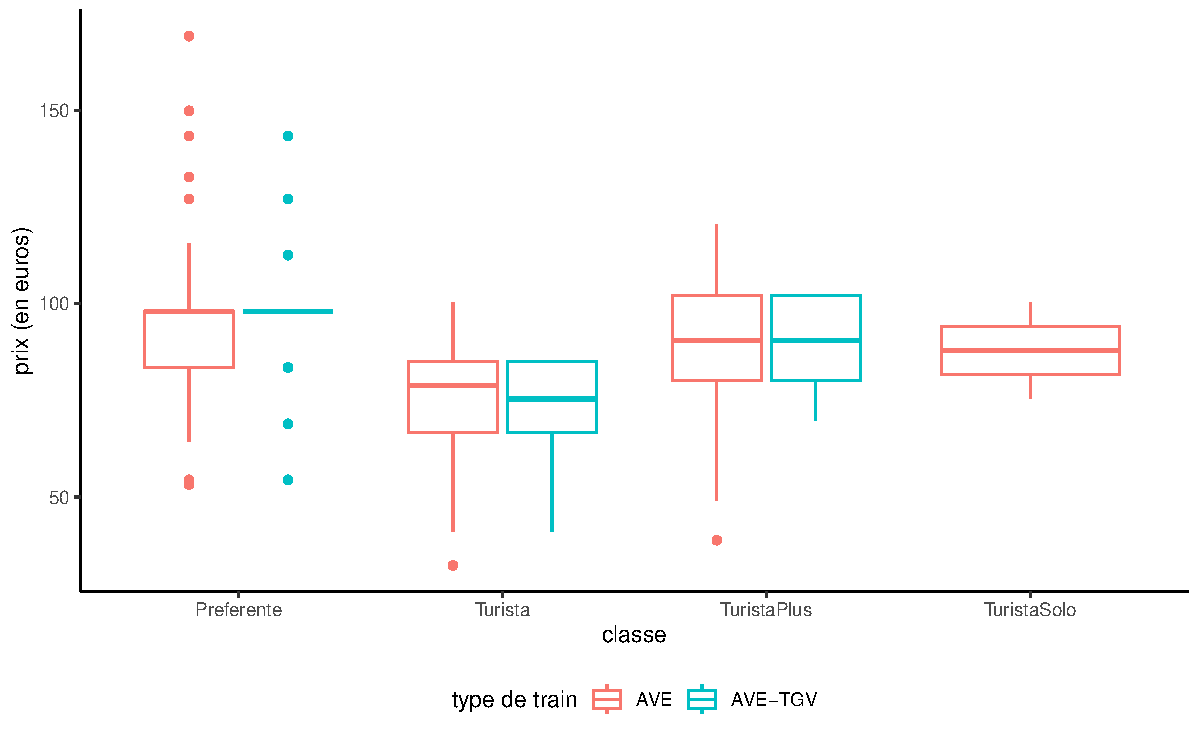
\includegraphics[width=0.85\textwidth,height=\textheight]{introduction_files/figure-pdf/fig-histboxplot-1.pdf}

}

\caption{\label{fig-histboxplot}Boîte à moustaches du prix des billets
au tarif Promo en fonction de la classe pour le jeu de données Renfe.}

\end{figure}%

Si on veut représenter la covariabilité de deux variables continues, on
utilise un nuage de points où chaque variable est représentée sur un axe
et chaque observation donne la coordonnée des points. Si la
représentation graphique est dominée par quelques valeurs très grandes,
une transformation des données peut être utile: vous verrez souvent des
données positives à l'échelle logarithmique. Si le nombre d'observations
est très grand, il devient difficile de distinguer quoi que ce soit. On
peut alors ajouter de la transparence ou regrouper des données en
compartiments bidimensionnels (un histogramme bidimensionnel), dont la
couleur représente la fréquence de chaque compartiment. Le paneau gauche
de Figure~\ref{fig-nuagedepoints} montre un nuage de points de 100
observations simulées, tandis que celui de droite représente des
compartiments hexagonaux contenant 10 000 points.

\begin{figure}[ht!]

\centering{

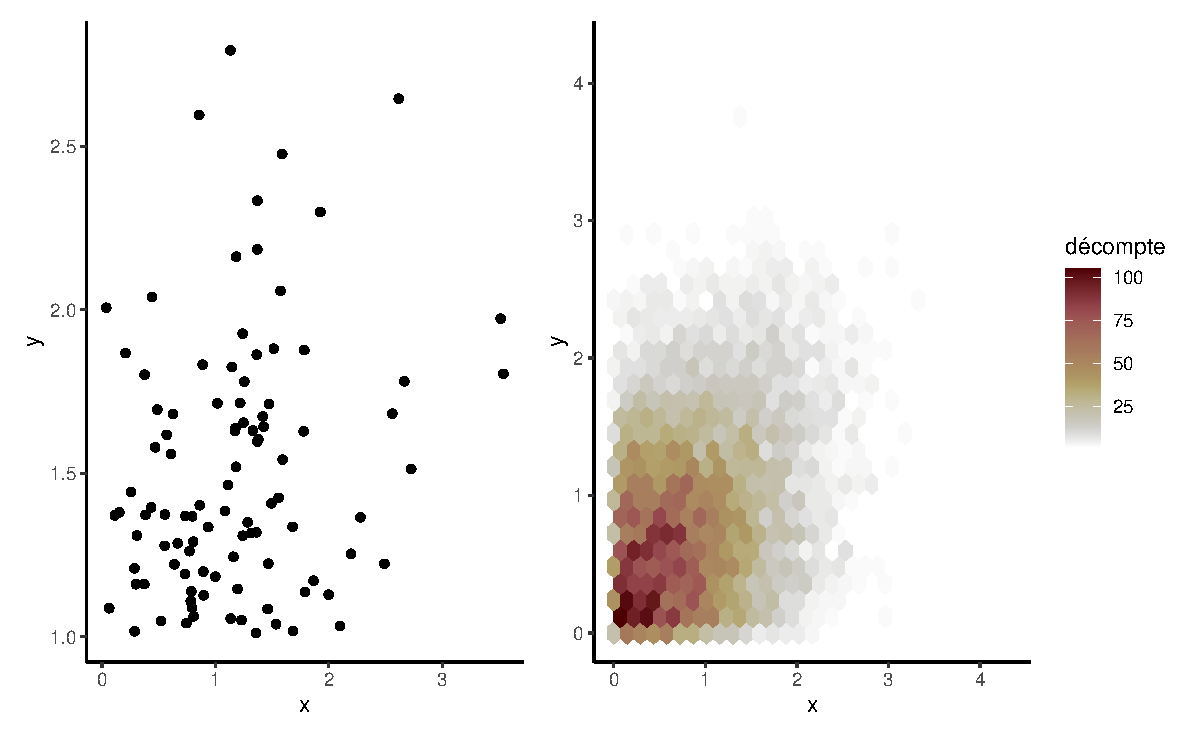
\includegraphics[width=0.85\textwidth,height=\textheight]{introduction_files/figure-pdf/fig-nuagedepoints-1.pdf}

}

\caption{\label{fig-nuagedepoints}Nuage de points (gauche) et diagramme
hexagonal (droite) pour des données simulées.}

\end{figure}%

Si on ajuste un modèle à des données, il convient de vérifier la qualité
de l'ajustement et l'adéquation du modèle, par exemple graphiquement.

\begin{definition}[Diagrammes
quantiles-quantiles]\protect\hypertarget{def-diagramme-qq}{}\label{def-diagramme-qq}

Le diagramme quantile-quantile sert à vérifier l'adéquation du modèle et
découle du constat suivant: si \(Y\) est une variable aléatoire continue
et \(F\) sa fonction de répartition, alors l'application
\(F(Y) \sim \mathsf{unif}(0,1)\), une loi uniforme standard. De la même
façon, appliquer la fonction quantile à une variable uniforme permet de
simuler de la loi \(F\), et donc \(F^{-1}(U)\). Supposons un échantillon
uniforme de taille \(n\). On peut démontrer que, pour des variables
continues, les statistiques d'ordre \(U_{(1)} \leq \cdots \leq U_{(n)}\)
ont une loi marginale beta, avec
\(U_{(k)} \sim \mathsf{Beta}(k, n+1-k)\) d'espérance \(k/(n+1)\).

Les paramètres de la loi \(F\) sont inconnus, mais on peut obtenir un
estimateur \(\widehat{F}\) et appliquer la transformation inverse pour
obtenir une variable approximativement uniforme. Un diagramme
quantile-quantile représente les données en fonction des moments des
statistiques d'ordre transformées

\begin{itemize}
\tightlist
\item
  sur l'axe des abscisses, les quantiles théoriques
  \(\widehat{F}^{-1}\{\mathrm{rang}(Y_i)/(n+1)\}\)
\item
  sur l'axe des ordonnées, les quantiles empiriques \(Y_i\)
\end{itemize}

Si le modèle est adéquat, les valeurs ordonnées devraient suivre une
droite de pente unitaire qui passe par l'origine. Le diagramme
probabilité-probabilité représente plutôt les données à l'échelle
uniforme \(\{\mathrm{rang}(Y_i)/(n+1), \widehat{F}(Y_i)\}\).

\end{definition}

\begin{figure}[ht!]

\centering{

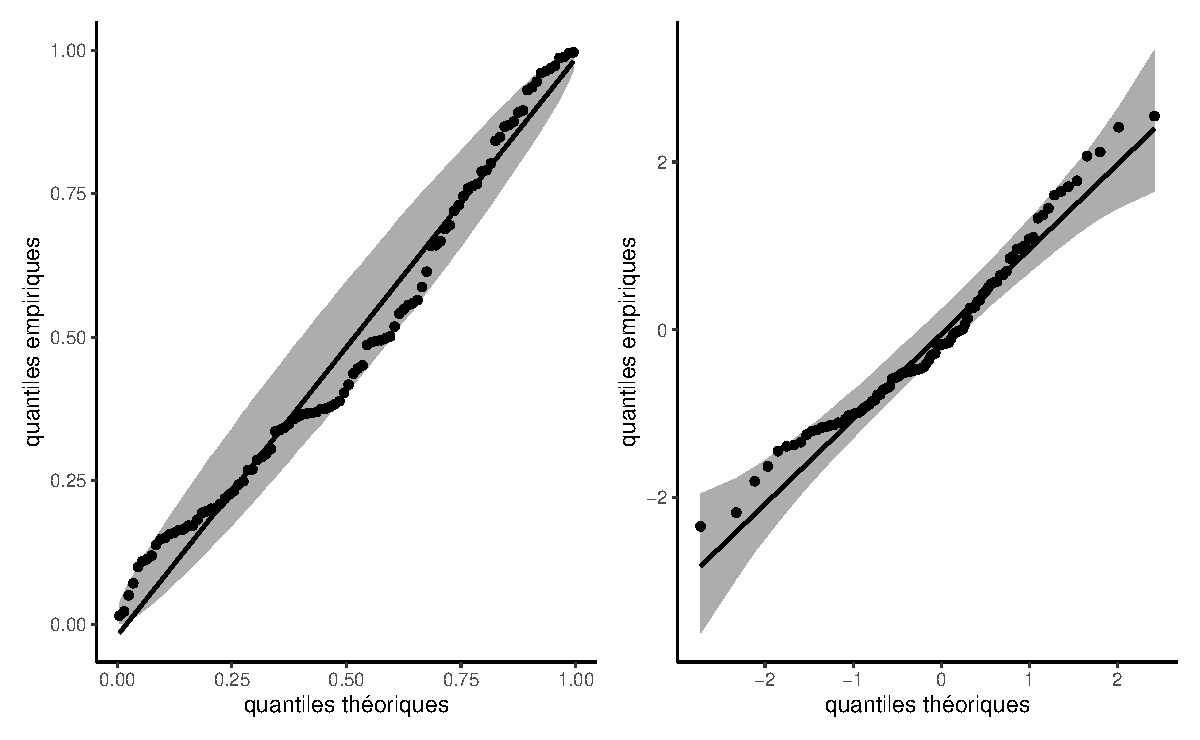
\includegraphics[width=0.85\textwidth,height=\textheight]{introduction_files/figure-pdf/fig-diagrammeqq2-1.pdf}

}

\caption{\label{fig-diagrammeqq2}Diagramme probabilité-probabilité
(gauche) et quantile-quantile normal (droite)}

\end{figure}%

Même si on connaissait exactement la loi aléatoire des données, la
variabilité intrinsèque à l'échantillon fait en sorte que des déviations
qui semblent significatives et anormales à l'oeil de l'analyste sont en
fait compatibles avec le modèle: un simple estimé ponctuel sans mesure
d'incertitude ne permet donc pas facilement de voir ce qui est plausible
ou pas. On va donc idéalement ajouter un intervalle de confiance
(approximatif) ponctuel ou conjoint au diagramme.

Pour obtenir l'intervalle de confiance approximatif, la méthode la plus
simple est par simulation, en répétant \(B\) fois les étapes suivantes

\begin{enumerate}
\def\labelenumi{\arabic{enumi}.}
\tightlist
\item
  simuler un échantillon \(\{Y^{(b)}_{i}\} (i=1,\ldots, n)\) du modèle
  \(\widehat{F}\)
\item
  estimer les paramètres du modèle \(F\) pour obtenir
  \(\widehat{F}_{(b)}\)
\item
  calculer et stocker les positions
  \(\widehat{F}^{-1}_{(b)}\{i/(n+1)\}\).
\end{enumerate}

Le résultat de cette opération sera une matrice \(n \times B\) de
données simulées; on obtient un intervalle de confiance symmétrique en
conservant le quantile \(\alpha/2\) et \(1-\alpha/2\) de chaque ligne.
Le nombre de simulation \(B\) devrait être large (typiquement 999 ou
davantage) et être choisi de manière à ce que \(B/\alpha\) soit un
entier.

Pour l'intervalle de confiance ponctuel, chaque valeur représente une
statistique et donc individuellement, la probabilité qu'une statistique
d'ordre sorte de l'intervalle de confiance est \(\alpha\). En revanche,
les statistiques d'ordres ne sont pas indépendantes et sont qui est plus
ordonnées, ce qui fait qu'un point hors de l'intervalle risque de n'être
pas isolé. Les intervalles présentés dans la
Figure~\ref{fig-diagrammeqq2} sont donc ponctuels. La variabilité des
statistiques d'ordre uniformes est plus grande autour de 1/2, mais
celles des variables transformées dépend de \(F\).

L'interprétation d'un diagramme quantile-quantile nécessite une bonne
dose de pratique et de l'expérience:
\href{https://stats.stackexchange.com/questions/101274/how-to-interpret-a-qq-plot/101290\#101290}{cette
publication par \emph{Glen\_b} sur StackOverflow} résume bien ce qu'on
peut détecter ou pas en lisant le diagramme.

\section{Loi des grands nombres}\label{loi-grands-nombres}

Un estimateur est dit \textbf{convergent} si la valeur obtenue à mesure
que la taille de l'échantillon augmente s'approche de la vraie valeur
que l'on cherche à estimer. Mathématiquement parlant, un estimateur est
dit convergent s'il converge en probabilité, ou
\(\hat{\theta} \stackrel{\mathsf{Pr}}{\to} \theta\): en langage commun,
la probabilité que la différence entre \(\hat{\theta}\) et \(\theta\)
diffèrent est négligeable quand \(n\) est grand.

La condition \emph{a minima} pour le choix d'un estimateur est donc la
convergence: plus on récolte d'information, plus notre estimateur
devrait s'approcher de la valeur qu'on tente d'estimer.

La loi des grands nombres établit que la moyenne empirique de \(n\)
observations indépendantes de même espérance, \(\overline{Y}_n\), tend
vers l'espérance commune des variables \(\mu\), où
\(\overline{Y}_n \rightarrow \mu\). En gros, ce résultat nous dit que
l'on réussit à approximer de mieux en mieux la quantité d'intérêt quand
la taille de l'échantillon (et donc la quantité d'information disponible
sur le paramètre) augmente. La loi des grands nombres est très utile
dans les expériences Monte Carlo: on peut ainsi approximer par
simulation la moyenne d'une fonction \(g(x)\) de variables aléatoires en
simulant de façon répétée des variables \(Y\) indépendantes et
identiquement distribuées et en prenant la moyenne empirique
\(n^{-1} \sum_{i=1}^n g(Y_i)\).

Si la loi des grands nombres nous renseigne sur le comportement limite
ponctuel, il ne nous donne aucune information sur la variabilité de
notre estimé de la moyenne et la vitesse à laquelle on s'approche de la
vraie valeur du paramètre.

\section{Théorème central limite}\label{TCL}

Le théorème central limite dit que, pour un échantillon aléatoire de
taille \(n\) dont les observations sont indépendantes et tirées d'une
loi quelconque d'espérance \(\mu\) et de variance finie \(\sigma^2\),
alors la moyenne empirique tend non seulement vers \(\mu\), mais à une
vitesse précise:

\begin{itemize}
\tightlist
\item
  l'estimateur \(\overline{Y}\) sera centré autour de \(\mu\),
\item
  l'erreur-type sera de \(\sigma/\sqrt{n}\); le taux de convergence est
  donc de \(\sqrt{n}\). Ainsi, pour un échantillon de taille 100,
  l'erreur-type de la moyenne empirique sera 10 fois moindre que
  l'écart-type de la variable aléatoire sous-jacente.
\item
  la loi approximative de la moyenne \(\overline{Y}\) sera normale.
\end{itemize}

Mathématiquement, le théorème central limite dicte que
\(\sqrt{n}(\overline{Y}-\mu) \stackrel{\mathrm{d}}{\rightarrow} \mathsf{normale}(0, \sigma^2)\).
Si \(n\) est grand (typiquement supérieur à \(30\), mais cette règle
dépend de la loi sous-jacente de \(Y\)), alors
\(\overline{Y} \stackrel{\cdot}{\sim} \mathsf{normale}(\mu, \sigma^2/n)\).

Comment interpréter ce résultat? On considère comme exemple le temps de
trajet moyen de trains à haute vitesse AVE entre Madrid et Barcelone
opérés par la Renfe.

\begin{figure}[ht!]

\centering{

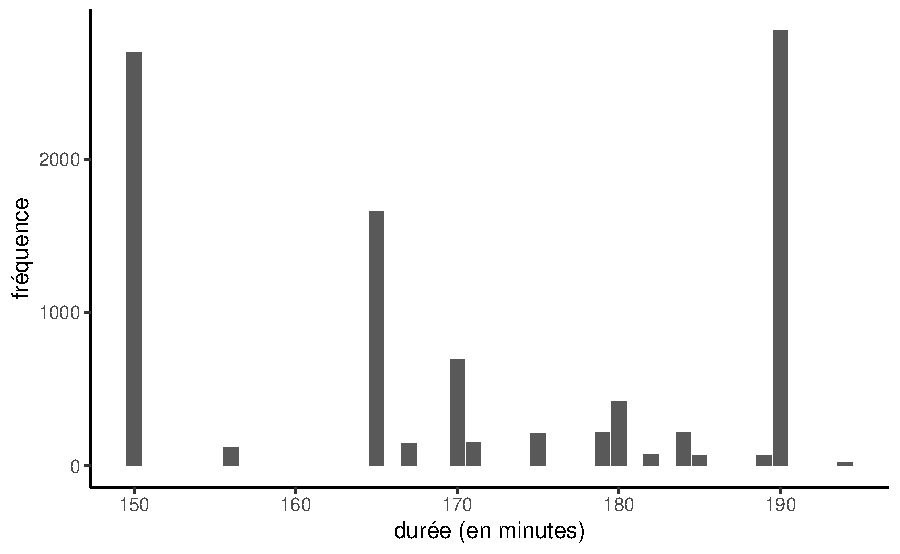
\includegraphics[width=0.85\textwidth,height=\textheight]{introduction_files/figure-pdf/fig-renfeclt-1.pdf}

}

\caption{\label{fig-renfeclt}Distribution empirique des temps de trajet
en trains à grande vitesse.}

\end{figure}%

Une analyse exploratoire indique que la durée du trajet de la base de
données est celle affichée sur le billet (et non le temps réel du
parcours). Ainsi, il n'y a ainsi que 15 valeurs possibles. Le temps
affiché moyen pour le parcours, estimé sur la base de 9603 observations,
est de 170 minutes et 41 secondes. La Figure~\ref{fig-renfeclt} montre
la distribution empirique des données.

Considérons maintenant des échantillons de taille \(n=10\). Dans notre
premier échantillon aléatoire, la durée moyenne affichée est 169.3
minutes, elle est de 167 minutes dans le deuxième, de 157.9 dans le
troisième, et ainsi de suite.

\begin{figure}[ht!]

\centering{

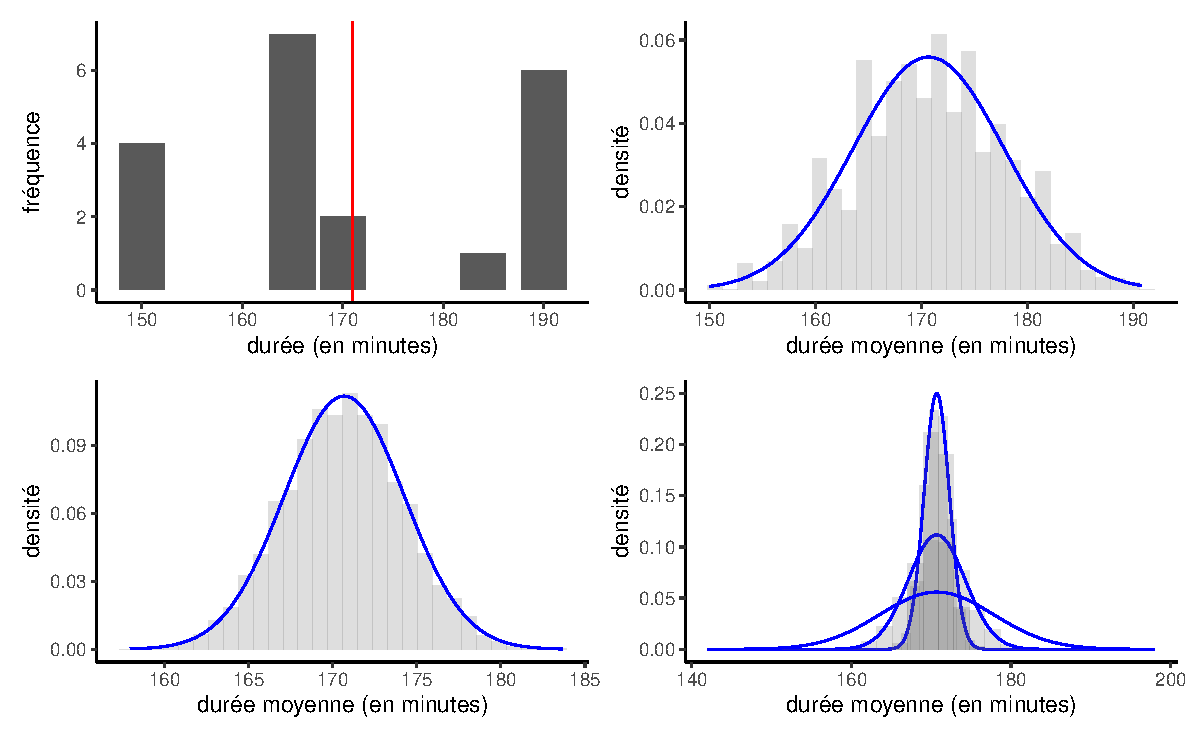
\includegraphics[width=0.9\textwidth,height=\textheight]{introduction_files/figure-pdf/fig-renfemeanCLT-1.pdf}

}

\caption{\label{fig-renfemeanCLT}Représentation graphique du théorème
central limite: échantillon aléatoire de 20 observations avec leur
moyenne empirique (trait vertical rouge) (en haut à gauche). Les trois
autres panneaux montrent les histogrammes des moyennes empiriques
d'échantillons répétés de taille 5 (en haut à droite), 20 (en bas à
gauche) et les histogrammes pour \(n=5, 20, 100\) (en bas à droite) avec
courbe de densité de l'approximation normale fournie par le théorème
central limite.}

\end{figure}%

Supposons qu'on tire \(B=1000\) échantillons différents, chacun de
taille \(n=5\), de notre ensemble, et qu'on calcule la moyenne de chacun
d'entre eux. Le graphique supérieur droit de la
Figure~\ref{fig-renfemeanCLT} montre un de ces 1000 échantillons
aléatoire de taille \(n=20\) tiré de notre base de données. Les autres
graphiques de la Figure~\ref{fig-renfemeanCLT} illustrent l'effet de
l'augmentation de la taille de l'échantillon: si l'approximation normale
est approximative avec \(n=5\), la distribution des moyennes est
virtuellement identique à partir de \(n=20\). Plus la moyenne est
calculée à partir d'un grand échantillon (c'est-à-dire, plus \(n\)
augmente), plus la qualité de l'approximation normale est meilleure et
plus la courbe se concentre autour de la vraie moyenne; malgré le fait
que nos données sont discrètes, la distribution des moyennes est
approximativement normale.

On a considéré une seule loi aléatoire inspirée de l'exemple, mais vous
pouvez vous amuser à regarder l'effet de la distribution sous-jacent et
de la taille de l'échantillon nécessaire pour que l'effet du théorème
central limite prenne effet: il suffit pour cela de simulant des
observations d'une loi quelconque de variance finie, en utilisant par
exemple cette
\href{http://195.134.76.37/applets/AppletCentralLimit/Appl_CentralLimit2.html}{applette}.

Les statistiques de test qui découlent d'une moyenne centrée-réduite (ou
d'une quantité équivalente pour laquelle un théorème central limite
s'applique) ont souvent une loi nulle standard normale, du moins
asymptotiquement (quand \(n\) est grand, typiquement \(n>30\) est
suffisant). C'est ce qui garantie la validité de notre inférence!

\bookmarksetup{startatroot}

\chapter{Inférence statistique}\label{inference}

Dans la plupart des domaines scientifiques, les donnéese empiriques
issues d'expériences contribuent à l'édification de la science. Afin de
tirer des conclusions en faveur ou à l'encontre d'une théorie, les
chercheurs se tournent (souvent à contrecoeur) vers la statistique. Cela
a conduit à la prédominance de l'utilisation du cadre des tests
statistiques et à la prépondérance des valeurs-\(p\) dans les articles
scientifiques, souvent employées de manière abusive ou fautive dans les
articles de journaux. La falsification d'une hypothèse nulle n'est pas
suffisante pour fournir des résultats substantiels pour une théorie.

Comme les cours d'introduction aux statistiques présentent généralement
des tests d'hypothèses sans accorder beaucoup d'attention aux principes
de construction sous-jacents de ces procédures, les utilisateurs ont
souvent une vision réductrice des statistiques. Plusieurs voient les
statistiques comme un catalogue de procédures pré-établies. Pour faire
une analogie culinaire, les utilisateurs se concentrent sur
l'apprentissage en vase clos des recettes plutôt que d'essayer de
comprendre les bases de la cuisine et de faire des liens. Ce chapitre se
concentre sur la compréhension des concepts-clés liées aux tests.

\begin{tcolorbox}[enhanced jigsaw, coltitle=black, bottomtitle=1mm, left=2mm, rightrule=.15mm, colback=white, bottomrule=.15mm, colframe=quarto-callout-important-color-frame, breakable, leftrule=.75mm, toprule=.15mm, titlerule=0mm, opacityback=0, title=\textcolor{quarto-callout-important-color}{\faExclamation}\hspace{0.5em}{Objectifs d'apprentissage}, opacitybacktitle=0.6, arc=.35mm, toptitle=1mm, colbacktitle=quarto-callout-important-color!10!white]

\begin{itemize}
\tightlist
\item
  Comprendre le rôle de l'incertitude dans la prise de décision.
\item
  Comprendre l'importance du rapport signal/bruit en tant que preuve.
\item
  Connaître les ingrédients de base des tests d'hypothèse et être
  capable de formuler et d'identifier correctement ces composants dans
  un article scientifique
\item
  Interpréter correctement les valeurs-\(p\) et les intervalles de
  confiance pour un paramètre.
\end{itemize}

\end{tcolorbox}

Avant d'entamer une collecte de données pour une expérience, il est
nécessaire de formuler une question de recherche. En général, cette
hypothèse spécifie les différences potentielles entre les
caractéristiques de la population dues à une intervention (un
traitement) que le chercheur souhaite quantifier. C'est à cette étape
que les chercheurs décident de la taille de l'échantillon, du choix de
la variable de réponse et de la méthode de mesure, qu'ils rédigent le
plan de l'étude, etc.

Il est important de noter que la plupart des questions de recherche ne
peuvent être résolues à l'aide d'outils simples. Les chercheurs qui
souhaitent mener une recherche méthodologique innovante devraient
contacter des experts et consulter des statisticien(ne)s \textbf{avant}
de collecter leurs données afin d'obtenir des informations sur la
meilleure façon de procéder pour ce qu'ils ont en tête, afin d'éviter le
risque d'affirmations trompeuses basées sur une analyse ou une collecte
de données incorrectes.

\begin{figure}[ht!]

\centering{

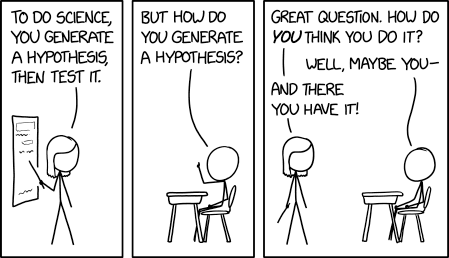
\includegraphics[width=0.6\textwidth,height=\textheight]{images/xkcd2569_hypothesis_generation.png}

}

\caption{\label{fig-xkcd2569}Bande dessinée xkcd
\href{https://xkcd.com/2569/}{2569 (Hypothesis generation) par Randall
Munroe}. Texte alternatif: Frazzled scientists are requesting that
everyone please stop generating hypotheses for a little bit while they
work through the backlog. Bande réimprimée sous license
\href{https://creativecommons.org/licenses/by-nc/2.5/}{CC BY-NC 2.5}.}

\end{figure}%

\section{Variabilité
échantillonale}\label{variabilituxe9-uxe9chantillonale}

Un chercheur s'intéressera à l'estimation de certaines caractéristiques
de la population à partir d'une base de données. Nous pouvons
caractériser l'ensemble de toutes les valeurs potentielles que leurs
mesures peuvent prendre, ainsi que leur fréquence, au moyen d'une loi
d'une variable aléatoire.

L'objectif de cette section est d'illustrer le fait que nous ne pouvons
pas simplement utiliser les différences brutes entre les groupes pour
effectuer des comparaisons significatives: en raison de la variabilité
due à l'échantillonnage, les échantillons seront semblables même s'ils
sont générés de la même manière, mais il y aura toujours des différences
entre les statistiques récapitulatives calculées sur des échantillons
différents. Ces différences ont tendance à s'atténuer (ou à augmenter)
au fur et à mesure que l'on collecte davantage d'observations. Plus nous
recueillons de données (et donc d'informations) sur notre cible, plus le
portrait devient précis. C'est somme toute ce qui nous permet de tirer
des conclusions mais, pour ce faire, nous devons d'abord déterminer ce
qui est probable ou plausible et donc le fruit du hsard, de ce qui n'est
pas ou peu susceptible de se produire.

Nous appelons \textbf{statistiques} les résumés numériques des données.
Il est important de faire la distinction entre les procédures ou
formules et leurs valeurs numériques. Un \textbf{estimateur} est une
règle ou une formule utilisée pour calculer une estimation d'un
paramètre ou d'une quantité d'intérêt sur la base de données observées
(comme une recette de gâteau). Une fois que nous disposons de données
observées, nous pouvons calculer la moyenne de l'échantillon,
c'est-à-dire que nous disposons d'une estimation --- d'une valeur réelle
(le gâteau), qui est une réalisation unique et non aléatoire. En
d'autres termes,

\begin{itemize}
\tightlist
\item
  un estimand est notre cible conceptuelle, comme la caractéristique de
  la population qui nous intéresse (la moyenne de la population).
\item
  un estimateur est la procédure ou la formule qui nous indique comment
  transformer les données de l'échantillon en un résumé numérique qui
  est une approximation de notre cible.
\item
  une estimation (ou un estimé) est un nombre, la valeur numérique
  obtenue lorsque nous appliquons la formule à un échantillon en
  praticulier.
\end{itemize}

\begin{figure}[ht!]

\begin{minipage}{0.33\linewidth}

\centering{


\includegraphics[width=0.85\textwidth,height=\textheight]{images/estimand.jpg}

}

\subcaption{\label{fig-cake-1}Estimand}

\end{minipage}%
%
\begin{minipage}{0.33\linewidth}

\centering{

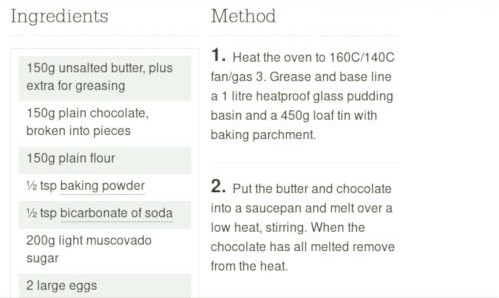
\includegraphics[width=0.85\textwidth,height=\textheight]{images/estimator.jpg}

}

\subcaption{\label{fig-cake-2}Estimateur}

\end{minipage}%
%
\begin{minipage}{0.33\linewidth}

\centering{

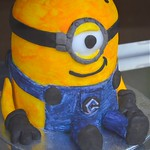
\includegraphics[width=0.85\textwidth,height=\textheight]{images/estimate.jpg}

}

\subcaption{\label{fig-cake-3}Estimé}

\end{minipage}%

\caption{\label{fig-cake}Les concepts
d'\href{https://www.flickr.com/photos/darkdwarf/16563489881}{estimand}
(gauche), estimateur (milieu) et
\href{https://www.flickr.com/photos/bensutherland/14685548773}{estimaté}
(droite), illustrés à l'aide de gâteau, une variation d'un idée
originale de Simon Grund. Les photos de gâteau sont partagées sous
licence \href{https://creativecommons.org/licenses/by-nc/2.0/}{CC BY-NC
2.0}.}

\end{figure}%

Par exemple, si l'estimand est l'espérance de la population \(\mu,\)
l'estimateur sera la moyenne arithmétique, soit la somme des éléments de
l'échantillon aléatoire divisé par la taille de l'échantillon, ou,
\(\overline{Y}=(Y_1 + \cdots + Y_n)/n.\) L'estimé sera une valeur
numérique, disons 4.3.

Parce que les intrants de l'estimateur sont aléatoires, la sortie l'est
également et varie d'un échantillon à l'autre. Autrement dit, même si on
répète une recette, on n'obtient pas le même résultat à chaque coup,
comme le montre si bien la Figure~\ref{fig-xkcd605}.

\begin{figure}[ht!]

\centering{

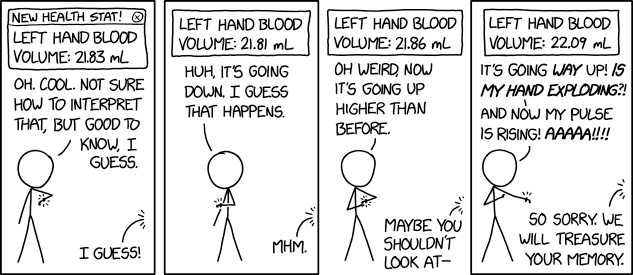
\includegraphics[width=0.7\textwidth,height=\textheight]{images/xkcd2581_health_stats.png}

}

\caption{\label{fig-xkcd605}Bande dessinée xkcd
\href{https://xkcd.com/2581/}{2581 (Health Stats) par Randall Munroe}.
Texte alternatif: You will live on forever in our hearts, pushing a
little extra blood toward our left hands now and then to give them a
squeeze. Bande réimprimée sous license
\href{https://creativecommons.org/licenses/by-nc/2.5/}{CC BY-NC 2.5}.}

\end{figure}%

Pour illustrer ce point, Figure~\ref{fig-samplevar} montre cinq
échantillons aléatoires simples de taille \(n=10\) tirés d'une
population hypothétique de moyenne théorique \(\mu\) et d'écart-type
\(\sigma,\) ainsi que leur moyenne d'échantillon \(\overline{y}.\) En
raison de la variabilité échantillonnale, les moyennes des sous-groupes
sont différentes même si elles proviennent de la même population. Vous
pouvez considérer la variabilité d'échantillonnage comme du bruit: notre
objectif est d'extraire le signal (typiquement les différences de
moyennes) tout en tenant compte du bruit de fond.

\begin{figure}[ht!]

\centering{

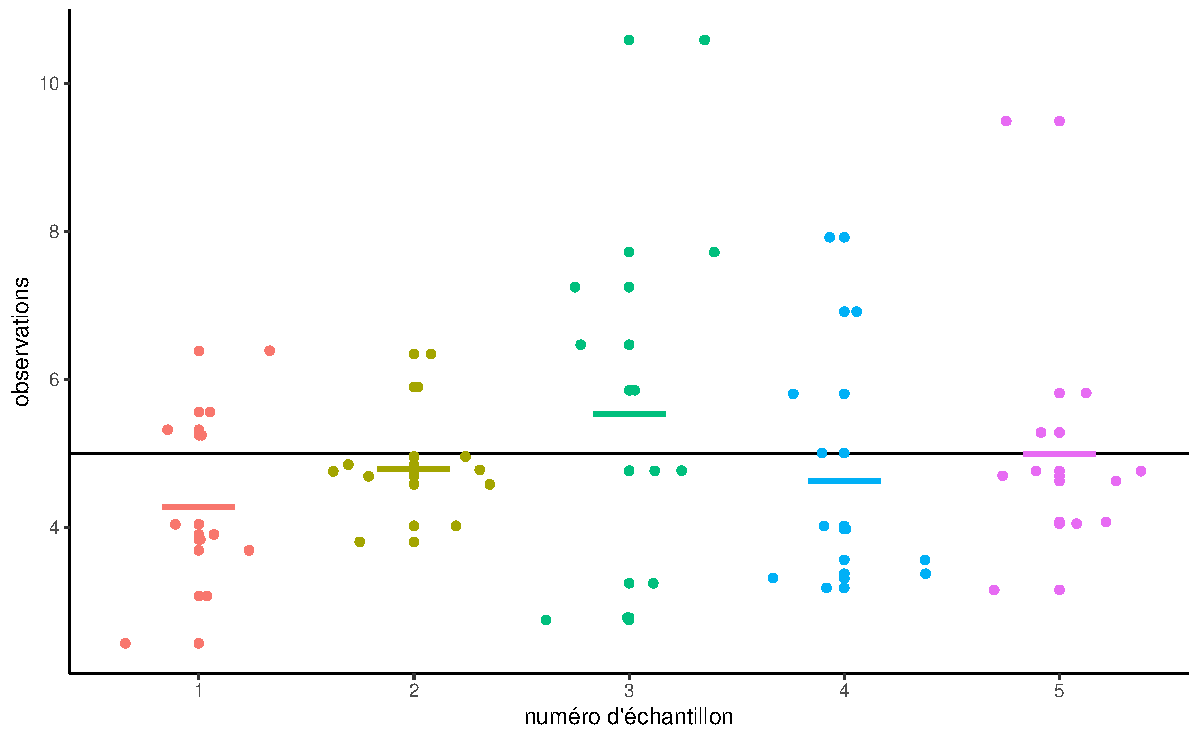
\includegraphics[width=0.85\textwidth,height=\textheight]{inference_files/figure-pdf/fig-samplevar-1.pdf}

}

\caption{\label{fig-samplevar}Cinq échantillons de taille \(n=10\) tirés
d'une population commune de moyenne \(\mu\) (ligne horizontale). Les
segments colorés représentent les moyennes empiriques de chaque groupe.}

\end{figure}%

L'oeil avisé pourra remarquer que les moyennes des cinq échantillons
(segments horizontaux colorés) sont moins dispersées autour de la ligne
horizontale noire représentant la moyenne de la population \(\mu\) que
ne le sont les observations. Il s'agit là d'un principe fondamental de
la statistique: l'information s'accumule au fur et à mesure que l'on
obtient plus de données.

Les valeurs de la moyenne de l'échantillon ne donnent pas une image
complète et l'étude des différences de moyenne (entre les groupes ou par
rapport à une valeur de référence postulée) n'est pas suffisante pour
tirer des conclusions. Dans la plupart des cas, rien ne garantit que la
moyenne de l'échantillon sera égale à sa valeur réelle, car elle varie
d'un échantillon à l'autre: la seule garantie que nous ayons est qu'elle
sera en moyenne égale à la moyenne de la population dans des
échantillons répétés. Selon le choix de la mesure et la variabilité de
la population, il peut y avoir des différences considérables d'une
observation à l'autre, ce qui signifie que la différence observée peut
être un coup de chance.

Pour avoir une idée du degré de certitude d'une chose, nous devons
considérer la variabilité d'une observation \(Y_i.\) Cette variance
d'une observation tirée de la population est typiquement notée
\(\sigma^2\) et sa racine carrée, l'écart-type, par \(\sigma.\)

L'écart-type \emph{d'une statistique} est appelé \textbf{erreur-type};
il ne doit pas être confondu avec l'écart-type \(\sigma\) de la
population dont sont tirées les observations de l'échantillon
\(Y_1, \ldots, Y_n.\) L'écart-type et l'erreur-type sont exprimés dans
les mêmes unités que les données et sont donc plus faciles à interpréter
que la variance. L'erreur-type étant fonction de la taille de
l'échantillon, il est d'usage de rapporter plutôt l'écart-type dans les
rapports.

\begin{example}[Proportion échantillonale et tirages
uniformes]\protect\hypertarget{exm-samppropunif}{}\label{exm-samppropunif}

Pour illustrer le concept de variabilité échantillonnale, nous suivons
l'exemple de {[}Matthew Crump{]}
(https://www.crumplab.com/statistics/foundations-for-inference.html) et
considérons des échantillons provenant d'une distribution uniforme sur
\(\{1, 2, \ldots, 10\}\): chaque entier de cet intervalle a la même
probabilité d'être tiré.

\begin{figure}[ht!]

\centering{

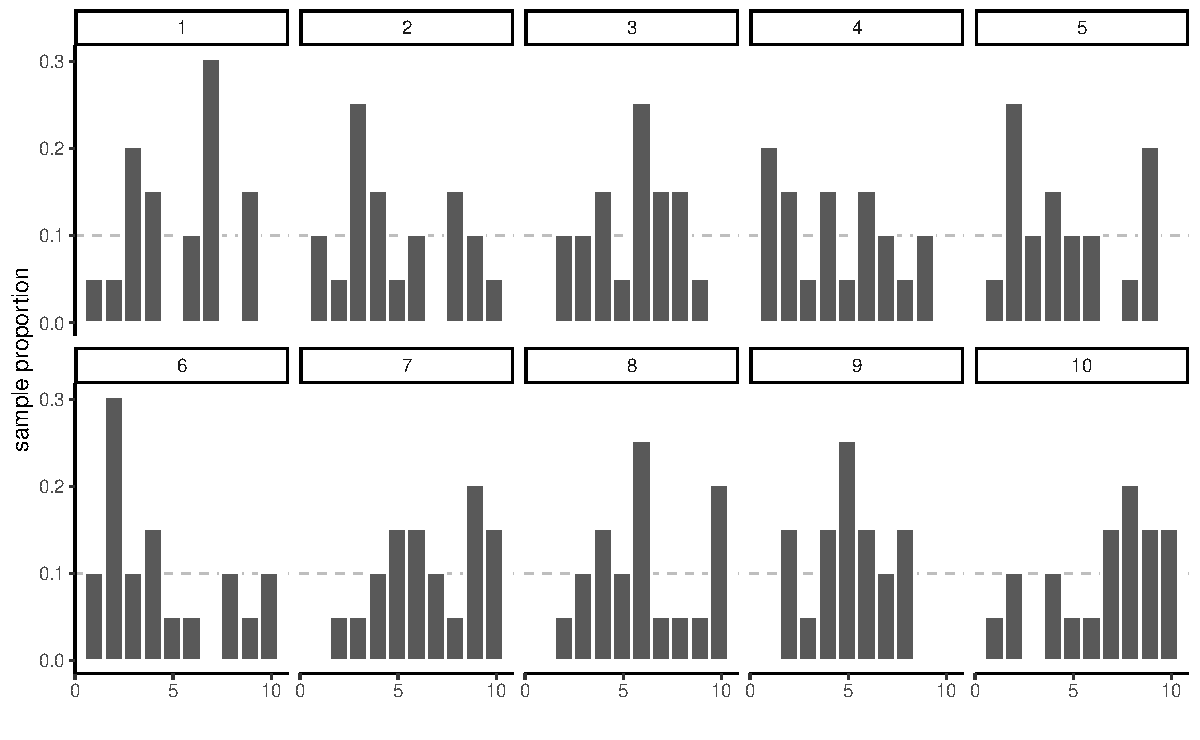
\includegraphics[width=0.85\textwidth,height=\textheight]{inference_files/figure-pdf/fig-unifsamp1-1.pdf}

}

\caption{\label{fig-unifsamp1}Histogrammes de 10 échantillons aléatoires
de taille \(n=20\) de loi uniforme discrète.}

\end{figure}%

Même s'ils sont tirés de la même population, les 10 échantillons de
Figure~\ref{fig-unifsamp1} sont très différents. La seule chose en jeu
ici est la variabilité de l'échantillon: puisqu'il y a \(n=20\)
d'observations au total, il devrait y avoir en moyenne 10\% des
observations dans chacun des 10 bacs, mais certains bacs sont vides et
d'autres ont plus d'effectifs que prévu. Cette fluctuation est le fruit
du hasard.

Comment pouvons-nous donc déterminer si ce que nous voyons est
compatible avec le modèle qui, selon nous, a généré les données ? Il
suffit de collecter davantage d'observations: la hauteur de la barre est
la proportion de l'échantillon, une moyenne de valeurs 0/1, où la valeur
`un' indique que l'observation se trouve dans la case, et `zéro' dans le
cas contraire.

Considérons maintenant ce qui se passe lorsque nous augmentons la taille
de l'échantillon: le panneau supérieur de Figure~\ref{fig-uniformsamp2}
montre des échantillons uniformes pour une taille d'échantillon
croissante. Le diagramme à bande ressemble de plus en plus à la
véritable distribution sous-jacente (fonction de masse constante, donc
chaque case ayant la même fréquence) à mesure que la taille de
l'échantillon augmente. La distribution des points de l'échantillon est
presque indiscernable de la distribution théorique (ligne droite)
lorsque \(n=10 000.\)\footnote{La formule montre que l'erreur standard
  diminue d'un facteur 10 chaque fois que la taille de l'échantillon
  augmente d'un facteur 100.}. Le panneau du bas, en revanche, ne
provient pas d'une distribution uniforme. Plus l'échantillon grossit,
plus l'approximation de la fonction de masse se rapproche de la vraie
valeur. Nous n'aurions pas pu remarquer cette différence dans les deux
premiers graphiques, car la variabilité de l'échantillonnage est trop
importante; là, le manque de données dans certaines cases pourrait être
un obstacle à l'obtention d'une distribution uniforme.

\begin{figure}[ht!]

\centering{

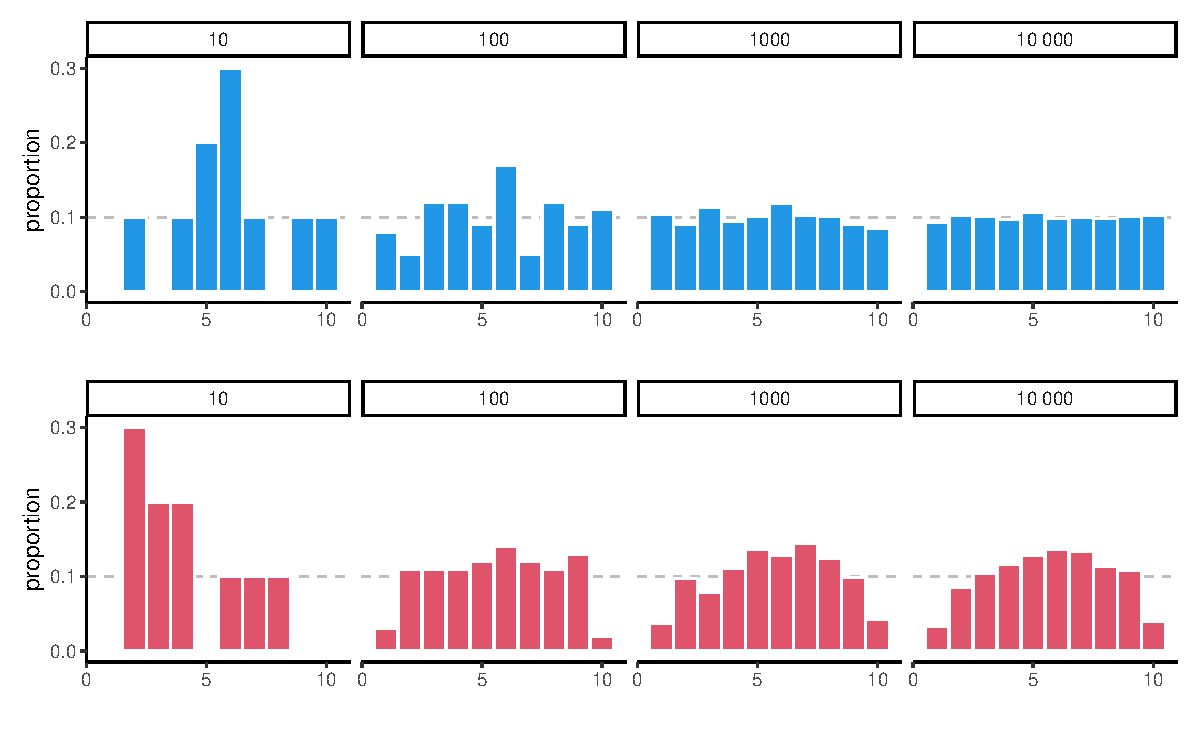
\includegraphics[width=0.85\textwidth,height=\textheight]{inference_files/figure-pdf/fig-uniformsamp2-1.pdf}

}

\caption{\label{fig-uniformsamp2}Histogrammes de données tirées d'une
loi uniforme (haut) et d'une loi non-uniforme (bas) pour des tailles
d'échantillons de 10, 100, 1000 and 10 000 (de gauche à droite).}

\end{figure}%

\end{example}

\section{Tests d'hypothèse}\label{tests}

Un test d'hypothèse statistique est une façon d'évaluer la preuve
statistique provenant d'un échantillon afin de faire une décision quant
à la population sous-jacente. Les étapes principales sont:

\begin{itemize}
\tightlist
\item
  définir les paramètres du modèle,
\item
  formuler les hypothèses alternative et nulle,
\item
  choisir et calculer la statistique de test,
\item
  déterminer son comportement sous \(\mathscr{H}_0\) (loi nulle),
\item
  calculer la valeur-\emph{p},
\item
  conclure dans le contexte du problème (rejeter ou ne pas rejeter
  \(\mathscr{H}_0\)).
\end{itemize}

Mon approche privilégiée pour présenter les tests d'hypothèse est de
faire un parallèle avec un procès pour meurtre où vous êtes nommé juré.

\begin{itemize}
\tightlist
\item
  Le juge vous demande de choisir entre deux hypothèses mutuellement
  exclusives, coupable ou non-coupable, sur la base des preuves
  présentées.
\item
  Votre postulat de départ repose sur la présomption d'innocence: vous
  condamnerez uniquement le suspect si la preuve est accablante. Cela
  permet d'éviter les erreurs judiciaires. L'hypothèse nulle
  \(\mathscr{H}_0\) est donc \emph{non-coupable}, et l'hypothèse
  alternative \(\mathscr{H}_a\) est coupable. En cas de doute
  raisonnable, vous émettrez un verdict de non-culpabilité.
\item
  La choix de la statistique de test représente la preuve. Plus la
  preuve est accablante, plus grande est la chance d'un verdict de
  culpabilité --- le procureur a donc tout intérêt à bien choisir les
  faits présentés en cour. Le choix de la statistique devrait donc
  idéalement maximiser la preuve pour appuyer le postulat de culpabilité
  le mieux possible (ce choix reflète la \textbf{puissance} du test).
\item
  En qualité de juré, vous analysez la preuve à partir de la
  jurisprudence et de l'avis d'expert pour vous assurer que les faits ne
  relèvent pas du hasard. Pour le test d'hypothèse, ce rôle est tenu par
  la loi sous \(\mathscr{H}_0\): si la personne était innocente, est-ce
  que les preuves présentées tiendraient la route? des traces d'ADN
  auront davantage de poids que des ouï-dire (la pièce de théâtre
  \emph{Douze hommes en colère} de Reginald Rose présente un bel exemple
  de procès où un des juré émet un doute raisonnable et convainc un à un
  les autres membres du jury de prononcer un verdict de
  non-culpabilité).
\item
  Vous émettez un verdict, à savoir une décision binaire, où l'accusé
  est déclaré soit non-coupable, soit coupable. Si vous avez une
  valeur-\emph{p}, disons \(P,\) pour votre statistique de test et que
  vous effectuez ce dernier à niveau \(\alpha,\) la règle de décision
  revient à rejeter \(\mathscr{H}_0\) si \(P < \alpha.\)
\end{itemize}

On s'attarde davantage sur ces définitions heuristiques et le
vocabulaire employé pour parler de tests d'hypothèse.

\section{Hypothèse}\label{hypothuxe8se}

Dans les test statistique il y a toujours deux hypothèse: l'hypothèse
nulle (\(\mathscr{H}_{0}\)) et l'hypothèse alternative
(\(\mathscr{H}_a\)). Habituellement, l'hypothèse nulle est le « statu
quo » et l'alternative est l'hypothèse que l'on cherche à démontrer. On
se fait l'avocat du Diable en défendant l'hypothèse nulle et en
analysant toutes les preuves sous l'angle: « est-ce que les données
entrent en contradiction avec \(\mathscr{H}_0\)? ». Un test d'hypothèse
statistique nous permet de décider si nos données nous fournissent assez
de preuves pour rejeter \(\mathscr{H}_0\) en faveur de
\(\mathscr{H}_a,\) selon un risque d'erreur spécifié.

Généralement, les tests d'hypothèses sont exprimés en fonction de
paramètres (de valeurs inconnues) du modèle sous-jacent, par ex.
\(\theta.\) Un test d'hypothèse bilatéral concernant un paramètre
scalaire \(\theta\) s'exprimerait la forme suivante: \begin{align*}
\mathscr{H}_0: \theta=\theta_0 \qquad \text{versus} \qquad \mathscr{H}_a:\theta \neq \theta_0.
\end{align*} Ces hypothèses permettent de tester si \(\theta\) est égal
à une valeur numérique précise \(\theta_0.\)

Par exemple, pour un test bilatéral concernant le paramètre d'un modèle
de régression \(\beta_j\) associé à une variable explicative d'intérêt
\(\mathrm{X}_j,\) les hypothèses sont \begin{align*}
\mathscr{H}_0: \beta_j=\beta_j^0 \qquad \text{versus} \qquad \mathscr{H}_a:\beta_j \neq \beta_j^0,
\end{align*} où \(\beta_j^0\) est une valeur précise qui est reliée à la
question de recherche. Par exemple, si \(\beta_j^0=0\) la question de
recherche sous-jacente est: est-ce que la covariable \(\mathrm{X}_j\)
impacte la variable réponse d'intérêt \(Y\) une fois l'effet des autres
variables pris en compte?

Il est possible d'imposer une direction dans les tests en considérant
une hypothèse alternative de la forme
\(\mathscr{H}_a: \theta > \theta_0\) ou
\(\mathscr{H}_a: \theta < \theta_0.\)

\section{Statistique de test}\label{statistique-de-test}

Une statistique de test \(T\) est une fonction des données qui résume
l'information contenue dans les données pour \(\theta.\) La forme de la
statistique de test est choisie de façon à ce que son comportement sous
\(\mathscr{H}_0,\) c'est-à-dire l'ensemble des valeurs que prend \(T\)
si \(\mathscr{H}_0\) est vraie et leur probabilité relative, soit connu.
En effet, \(T\) est une variable aléatoire et sa valeur va changer selon
l'échantillon. La \textbf{loi nulle} de la statistique de test nous
permet de déterminer quelles valeurs de \(T\) sont plausibles si
\(\mathscr{H}_0\) est vraie. Plusieurs statistiques que l'on couvrira
dans ce cours sont des \textbf{statistiques de Wald}, de la forme
\begin{align*}
T = \frac{\widehat{\theta} - \theta_0}{\mathrm{se}(\widehat{\theta})}
\end{align*} où \(\widehat{\theta}\) est l'estimateur du paramètre
\(\theta,\) \(\theta_0\) la valeur numérique postulée (par ex., zéro) et
\(\mathrm{se}(\widehat{\theta})\) est l'estimateur de l'écart-type de
\(\widehat{\theta}.\)

Par exemple, pour une hypothèse sur la moyenne d'une population de la
forme \begin{align*}
\mathscr{H}_0: \mu=0, \qquad  \mathscr{H}_a:\mu \neq 0,
\end{align*} la statistique de test de Wald est \begin{align*}
T &= \frac{\overline{X}-0}{S_n/\sqrt{n}}
\end{align*} où \(\overline{X}\) est la moyenne de l'échantillon
\(X_1, \ldots, X_n,\) \begin{align*}
\overline{X} &= \frac{1}{n} \sum_{i=1}^n X_i = \frac{X_1+ \cdots + X_n}{n}
\end{align*} et l'erreur-type de la moyenne \(\overline{X}\) est
\(S_n/\sqrt{n}\); l'écart-type \(S_n\) est un estimateur de \(\sigma,\)
où \begin{align*}
S^2_n &= \frac{1}{n-1} \sum_{i=1}^n (X_i-\overline{X})^2.
\end{align*}

\section{\texorpdfstring{Loi nulle et
valeur-\emph{p}}{Loi nulle et valeur-p}}\label{loi-nulle-et-valeur-p}

La \textbf{valeur-\emph{p}} nous permet de déterminer si la valeur
observée de la statistique de test \(T\) est plausible sous
\(\mathscr{H}_0.\) Plus précisément, la valeur-\emph{p} est la
probabilité, si \(\mathscr{H}_0\) est vraie, que la statistique de test
soit égale or plus extrême à ce qu'on observe. Supposons qu'on a un
échantillon \(X_1, \ldots, X_n\) et qu'on observe une valeur de la
statistique de test de \(T=t.\) Pour un test d'hypothèse bilatéral
\(\mathscr{H}_0:\theta=\theta_0\)
vs.~\(\mathscr{H}_a:\theta \neq \theta_0,\) la valeur-\emph{p} est
\(\Pr{\!}_0(|T| \geq |t|).\) Si la distribution de \(T\) est symétrique
autour de zéro, la valeur-\emph{p} vaut \begin{align*}
p = 2 \times \Pr{\!}_0(T \geq |t|).
\end{align*}

La Figure~\ref{fig-power-plots} montre la loi des valeurs-\(p\) sous
deux scénarios: à gauche, une loi nulle et à droite, une loi
alternative. La probabilité de rejetter \(\mathscr{H}_0\) est obtenue en
calculant l'aire sous la courbe sous la courbe de densité et
\(\alpha=0.1.\) Sous l'hypothèse nulle, le modèle est calibré et la loi
des valeurs-\(p\) est uniforme (un rectangle de hauteur 1), ce qui veut
dire que toutes les valeurs sont également plausibles. Sous
l'alternative, l'obtention de petites valeurs\(-\)p est plus plausible.

\begin{figure}[ht!]

\centering{

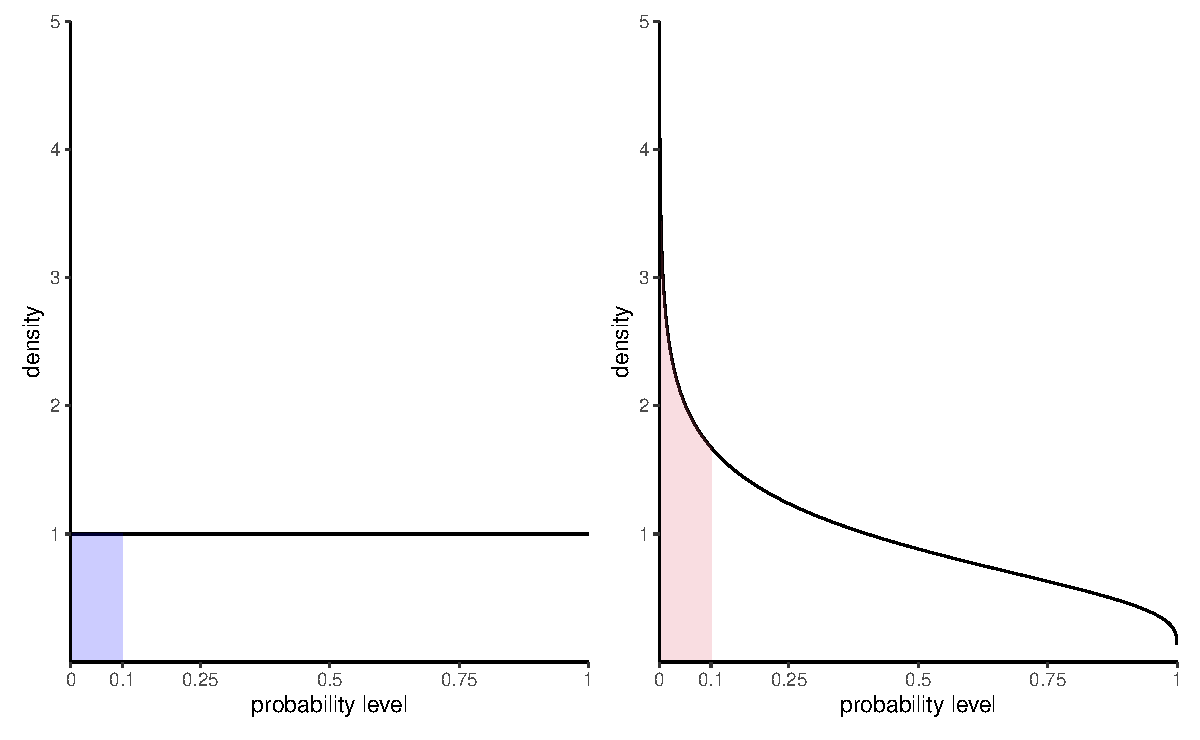
\includegraphics[width=0.85\textwidth,height=\textheight]{inference_files/figure-pdf/fig-power-plots-1.pdf}

}

\caption{\label{fig-power-plots}Densité des valeurs-\(p\) sou
l'hypothèse nulle (gauche) et une alternative avec un ratio signal-bruit
de 0.5 (droite).}

\end{figure}%

Il existe généralement trois façons d'obtenir des lois nulles pour
évaluer le degré de preuve contre l'hypothèse nulle

\begin{itemize}
\tightlist
\item
  les calculs exacts (combinatoires)
\item
  la théorie des grands échantillons (appelée « régime asymptotique »
  dans le jargon statistique)
\item
  les méthodes de simulation Monte Carlo.
\end{itemize}

Bien que souhaitable, la première méthode n'est applicable que dans des
cas simples (comme le calcul de la probabilité d'obtenir deux six en
lançant deux dés identiques). La deuxième méthode est la plus couramment
utilisée en raison de sa généralité et de sa facilité d'utilisation (en
particulier dans les temps anciens où la puissance de calcul était
rare), mais elle ne donne pas de bons résultats avec des échantillons de
petite taille (où la noti de « trop petit » dépend du contexte et du
test). La dernière approche peut être utilisée pour approcher la
distribution nulle dans de nombreux scénarios, mais elle ajoute une
couche d'aléatoire et les coûts de calcul supplémentaires n'en valent
parfois pas la peine.

Prenons l'exemple d'un test d'hypothèse bilatéral pour la moyenne au
population \(\mathscr{H}_0:\mu=0\) contre \(\mathscr{H}_a:\mu \neq 0.\)
Si l'échantillon provient d'une (population de) loi normale
\(\mathsf{normale}(\mu, \sigma^2),\) on peut démontrer que, si
\(\mathscr{H}_0\) est vraie et donc \(\mu=0\)), la statistique de test
\begin{align*}
T = \frac{\overline{X}}{S/\sqrt{n}}
\end{align*} suit une loi de Student-\(t\) avec \(n-1\) degrés de
liberté, dénotée \(\mathsf{Student}_{n-1}.\) À partir de cette loi
nulle, on peut calculer la valeur-\emph{p} (ou bien à partir d'une table
ou d'un logiciel statistique). Puisque la distribution Student-\(t\) est
symétrique autour de \(0,\) on peut calculer la valeur-\emph{p} comme
\(P = 2\times\Pr(T > |t|),\) où \(T \sim \mathsf{Student}_{n-1}.\)

\section{Intervalle de confiance}\label{intervalle-de-confiance}

Un \textbf{intervalle de confiance} est une manière alternative de
rapporter les conclusions d'un test, en ce sens qu'on fournit une
estimation ponctuelle de \(\hat{\theta}\) avec une marge d'erreur.
L'intervalle de confiance donne donc une indication de la variabilité de
la procédure d'estimation. Un intervalle de confiance de Wald à
\((1-\alpha)\) pour un paramètre \(\theta\) est de la forme
\begin{align*}
[\widehat{\theta} + \mathfrak{q}_{\alpha/2}\mathrm{se}(\widehat{\theta}), \widehat{\theta} +\mathfrak{q}_{1-\alpha/2}\times \mathrm{se}(\widehat{\theta})]
\end{align*} où \(\mathfrak{q}_{\alpha}\) dénote le quantile d'ordre
\(\alpha \in (0,1)\) de la loi nulle de la statistique de Wald,
\begin{align*}
T =\frac{\widehat{\theta}-\theta}{\mathrm{se}(\widehat{\theta})},
\end{align*} et où \(\theta\) représente la valeur du paramètre
\(\theta\) (supposé fixe, mais inconnu) de la population.

Par exemple, pour un échantillon aléatoire \(X_1, \ldots, X_n\)
provenant d'une loi \(\mathsf{normale}(\mu, \sigma),\) l'intervalle de
confiance à \((1-\alpha)\) pour la moyenne (dans la population) \(\mu\)
est \begin{align*}
\overline{X} \pm t_{n-1, \alpha/2} \frac{S}{\sqrt{n}}
\end{align*} où \(t_{n-1, \alpha/2}\) est le quantile d'ordre
\(1-\alpha/2\) de la loi Student-\(t\) avec \(n-1\) degrés de libertés.

Les bornes de l'intervalle de confiance sont aléatoires puisque
\(\widehat{\theta}\) et \(\mathrm{se}(\widehat{\theta})\) sont des
variable aléatoires: leurs valeurs observées changent d'un échantillon à
un autre. Avant qu'on calcule l'intervalle de confiance, il y a une
probabilité de \(1-\alpha\) que \(\theta\) soit contenu dans
l'intervalle \textbf{aléatoire} symmétrique
\((\widehat{\theta} - \mathfrak{q}_{\alpha/2} \; \mathrm{se}(\widehat{\theta}), \widehat{\theta} + \mathfrak{q}_{\alpha/2} \; \mathrm{se}(\widehat{\theta})),\)
où \(\widehat{\theta}\) dénote l'estimateur de \(\theta.\) Une fois
qu'on obtient un échantillon et qu'on calcule les bornes de l'intervalle
de confiance, il n'y a plus de notion de probabilité: la vraie valeur du
paramètre \(\theta\) (inconnue) est soit contenue dans l'intervalle de
confiance, soit pas. La seule interprétation de l'intervalle de
confiance qui soit valable alors est la suivante: si on répète
l'expérience plusieurs fois et qu'à chaque fois on calcule un intervalle
de confiance à \(1-\alpha,\) alors une proportion de \((1-\alpha)\) de
ces intervalles devraient contenir la vraie valeur de \(\theta\) (de la
même manière, si vous lancez une pièce de monnaie équilibrée, vous
devriez obtenir grosso modo une fréquence de 50\% de pile et 50\% de
face, mais chaque lancer donnera un ou l'autre de ces choix). Notre «
confiance » est dans la procédure et non pas dans les valeurs numériques
obtenues pour un échantillon donné.

\begin{figure}[ht!]

\centering{

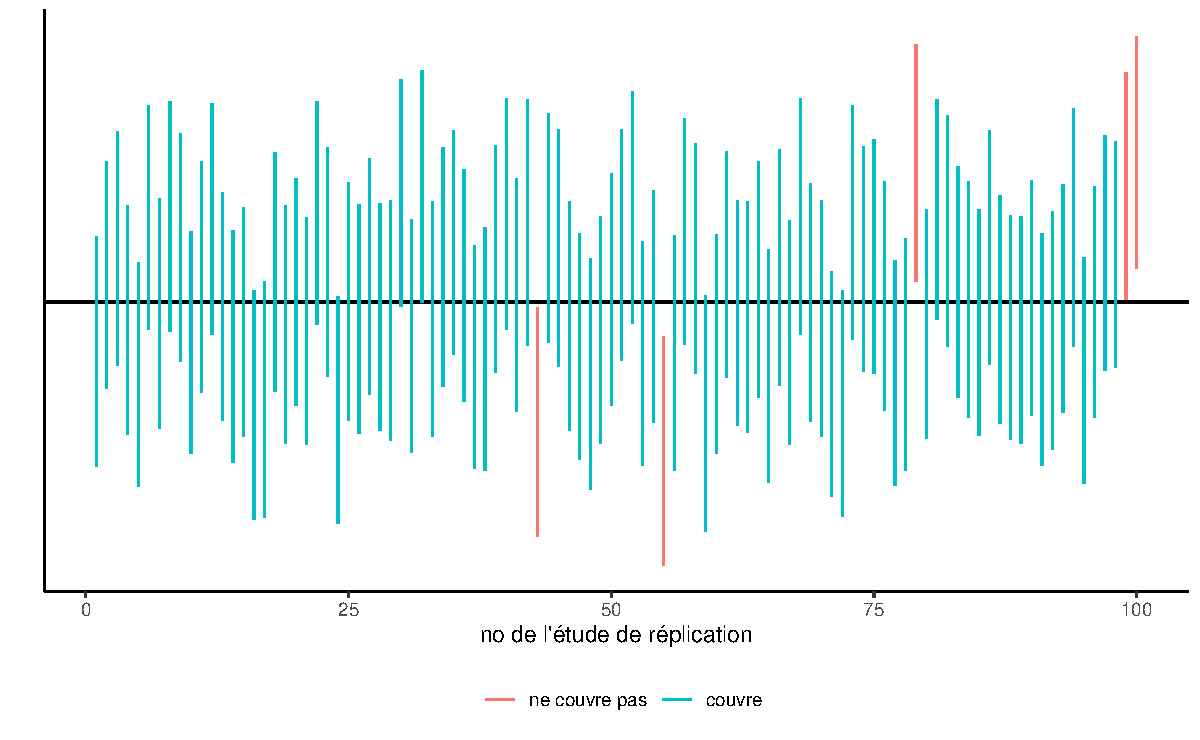
\includegraphics[width=0.85\textwidth,height=\textheight]{inference_files/figure-pdf/fig-intconf-1.pdf}

}

\caption{\label{fig-intconf}Intervalles de confiance à 95\% pour la
moyenne d'une population normale standard pour 100 échantillons
aléatoires. En moyenne, 5\% de ces intervalles (en rouge) n'incluent pas
la vraie valeur de la moyenne de zéro.}

\end{figure}%

Si on s'intéresse seulement à la décision rejeter/ne pas rejeter
\(\mathscr{H}_0,\) l'intervalle de confiance est équivalent à la
valeur-\emph{p} en ce sens qu'il mène à la même décision. L'intervalle
de confiance donne en revanche l'ensemble des valeurs pour lesquelles la
statistique de test ne fournit pas assez de preuves pour rejeter
\(\mathscr{H}_0\): pour un test à niveau \(\alpha,\) on ne rejetterait
aucune des valeurs contenues dans l'intervalle de confiance de niveau
\(1-\alpha.\) Si la valeur-\emph{p} est inférieure à \(\alpha,\) la
valeur postulée pour \(\theta\) est donc hors de l'intervalle de
confiance calculé. À l'inverse, la valeur-\emph{p} ne donne la
probabilité d'obtenir un résultat aussi extrême sous l'hypothèse nulle
que pour une seule valeur numérique, mais permet de quantifier
précisément à quel point le résultat est extrême.

\section{Conclusion}\label{conclusion}

La valeur-\emph{p} nous permet de faire une décision quant aux
hypothèses du test. Si \(\mathscr{H}_0\) est vraie, la valeur-\emph{p}
suit une loi uniforme. \href{https://xkcd.com/1478/}{Si la
valeur-\emph{p} est petite}, ça veut dire que le fait d'observer une
statistique de test égal ou encore plus extrême que \(T=t\) est peu
probable, et donc nous aurons tendance de croire que \(\mathscr{H}_0\)
n'est pas vraie. Il y a pourtant toujours un risque sous-jacent de
commettre un erreur quand on prend une décision. En statistique, il y a
\href{https://xkcd.com/2303/}{deux types d'erreurs}:

\begin{itemize}
\tightlist
\item
  erreur de type I: on rejette \(\mathscr{H}_0\) alors que
  \(\mathscr{H}_0\) est vraie
\item
  erreur de type II: on ne rejette pas \(\mathscr{H}_0\) alors que
  \(\mathscr{H}_0\) est fausse
\end{itemize}

Ces deux erreurs ne sont pas égales: on cherche souvent à contrôler
l'erreur de type I (une erreur judiciaire, condamner un innocent). Pour
se prémunir face à ce risque, on fixe préalablement un niveau de
tolérance. Plus notre seuil de tolérance \(\alpha\) est grand, plus on
rejette souvent l'hypothèse nulle même si cette dernière est vraie. La
valeur de \(\alpha \in (0, 1)\) est la probabilité qu'on rejette
\(\mathscr{H}_0\) quand \(\mathscr{H}_0\) est en fait vraie.
\begin{align*}
\alpha = \Pr{\!}_0\left(\text{ rejeter } \mathscr{H}_0\right).
\end{align*} Comme chercheur, on choisit ce niveau \(\alpha\);
habituellement \(1\)\%, \(5\)\% ou \(10\)\%. La probabilité de commettre
une erreur de type I est \(\alpha\) seulement si le modèle nul postulé
pour \(\mathscr{H}_0\) est correctement spécifié (sic) et correspond au
modèle générateur des données.

Le choix du statu quo (typiquement \(\mathscr{H}_0\)) s'explique plus
facilement avec un exemple médical. Si vous voulez prouver qu'un nouveau
traitement est meilleur que l'actuel (ou l'absence de traitement), vous
devez démontrer hors de tout doute raisonnable que ce dernier ne cause
pas de torts aux patients et offre une nette amélioration (pensez à
Didier Raoult et ses allégations non-étayées voulant que
l'hydrochloroquine, un antipaludique, soit efficace face au virus de la
Covid19).

\begin{longtable}[]{@{}
  >{\raggedright\arraybackslash}p{(\columnwidth - 4\tabcolsep) * \real{0.3333}}
  >{\centering\arraybackslash}p{(\columnwidth - 4\tabcolsep) * \real{0.3333}}
  >{\centering\arraybackslash}p{(\columnwidth - 4\tabcolsep) * \real{0.3333}}@{}}
\toprule\noalign{}
\begin{minipage}[b]{\linewidth}\raggedright
\textbf{Décision} \textbackslash{} \textbf{vrai modèle}
\end{minipage} & \begin{minipage}[b]{\linewidth}\centering
\(\mathscr{H}_0\)
\end{minipage} & \begin{minipage}[b]{\linewidth}\centering
\(\mathscr{H}_a\)
\end{minipage} \\
\midrule\noalign{}
\endhead
\bottomrule\noalign{}
\endlastfoot
ne pas rejeter \(\mathscr{H}_0\) & \(\checkmark\) & erreur de type II \\
rejeter \(\mathscr{H}_0\) & erreur de type I & \(\checkmark\) \\
\end{longtable}

Pour prendre une décision, on doit comparer la valeur-\emph{p} \(P\)
avec le niveau du test \(\alpha\):

\begin{itemize}
\tightlist
\item
  si \(P < \alpha\) on rejette \(\mathscr{H}_0,\)
\item
  si \(P \geq \alpha\) on ne rejette pas \(\mathscr{H}_0.\)
\end{itemize}

Attention à ne pas confondre niveau du test (probabilité fixée au
préalable par l'expérimentateur) et la valeur-\emph{p} (qui dépend de
l'échantillon). Si vous faites un test à un niveau 5\% la probabilité de
faire une erreur de type I est de 5\% par définition, quelque soit la
valeur de la valeur-\emph{p}. La valeur-\emph{p} s'interprète comme la
probabilité d'obtenir une valeur de la statistique de test égale ou même
plus grande que celle qu'on a observée dans l'échantillon, si
\(\mathscr{H}_0\) est vraie.

\begin{tcolorbox}[enhanced jigsaw, coltitle=black, bottomtitle=1mm, left=2mm, rightrule=.15mm, colback=white, bottomrule=.15mm, colframe=quarto-callout-caution-color-frame, breakable, leftrule=.75mm, toprule=.15mm, titlerule=0mm, opacityback=0, title=\textcolor{quarto-callout-caution-color}{\faFire}\hspace{0.5em}{Mise en garde}, opacitybacktitle=0.6, arc=.35mm, toptitle=1mm, colbacktitle=quarto-callout-caution-color!10!white]

L'\href{https://doi.org/10.1080/00031305.2016.1154108}{\emph{American
Statistical Association (ASA)} a publié une liste de principes}
détaillant les principales erreurs d'interprétation des valeurs-\(p,\)
notamment

\begin{quote}
\begin{enumerate}
\def\labelenumi{(\arabic{enumi})}
\setcounter{enumi}{1}
\tightlist
\item
  Les valeurs-\(p\) ne mesurent pas la probabilité que l'hypothèse
  étudiée est vrai
\end{enumerate}
\end{quote}

\begin{quote}
\begin{enumerate}
\def\labelenumi{(\arabic{enumi})}
\setcounter{enumi}{2}
\tightlist
\item
  Les décisions d'affaires et scientiques ne devraient pas seulement
  être basées sur le fait qu'une valeur-\(p\) est inférieure à un seuil
  spécifié.
\end{enumerate}
\end{quote}

\begin{quote}
\begin{enumerate}
\def\labelenumi{(\arabic{enumi})}
\setcounter{enumi}{3}
\tightlist
\item
  Les analyses statistiques et les valeurs-\(p\) associées ne devraient
  pas être rapportées de manière sélective.
\end{enumerate}
\end{quote}

\begin{quote}
\begin{enumerate}
\def\labelenumi{(\arabic{enumi})}
\setcounter{enumi}{4}
\tightlist
\item
  Les valeurs-\(p,\) ou la significativité statistiques, ne mesurent pas
  la taille de l'effet ou l'importance d'un résultat.
\end{enumerate}
\end{quote}

\end{tcolorbox}

\section{Puissance statistique}\label{puissance-statistique}

Le but du test d'hypothèse est de prouver (hors de tout doute
raisonnable) qu'une différence ou un effet est significatif: par
exemple, si une nouvelle configuration d'un site web (hypothèse
alternative) permet d'augmenter les ventes par rapport au statu quo.
Notre capacité à détecter cette amélioration dépend de la puissance du
test: plus cette dernière est élevée, plus grande est notre capacité à
rejeter \(\mathscr{H}_0\) quand ce dernier est faux.

Quand on ne rejette pas \(\mathscr{H}_0\) et que \(\mathscr{H}_a\) est
en fait vraie, on commet une erreur de type II: cette dernière survient
avec probabilité \(1-\gamma.\) La \textbf{puissance statistique} d'un
test est la probabilité que le test rejette \(\mathscr{H}_0\) alors que
\(\mathscr{H}_0\) est fausse, soit \begin{align*}
\gamma = \Pr{\!}_a(\text{rejeter } \mathscr{H}_0)
\end{align*} Selon le choix de l'alternative, il est plus ou moins
facile de rejeter l'hypothèse nulle en faveur de l'alternative.

\begin{figure}[ht!]

\centering{

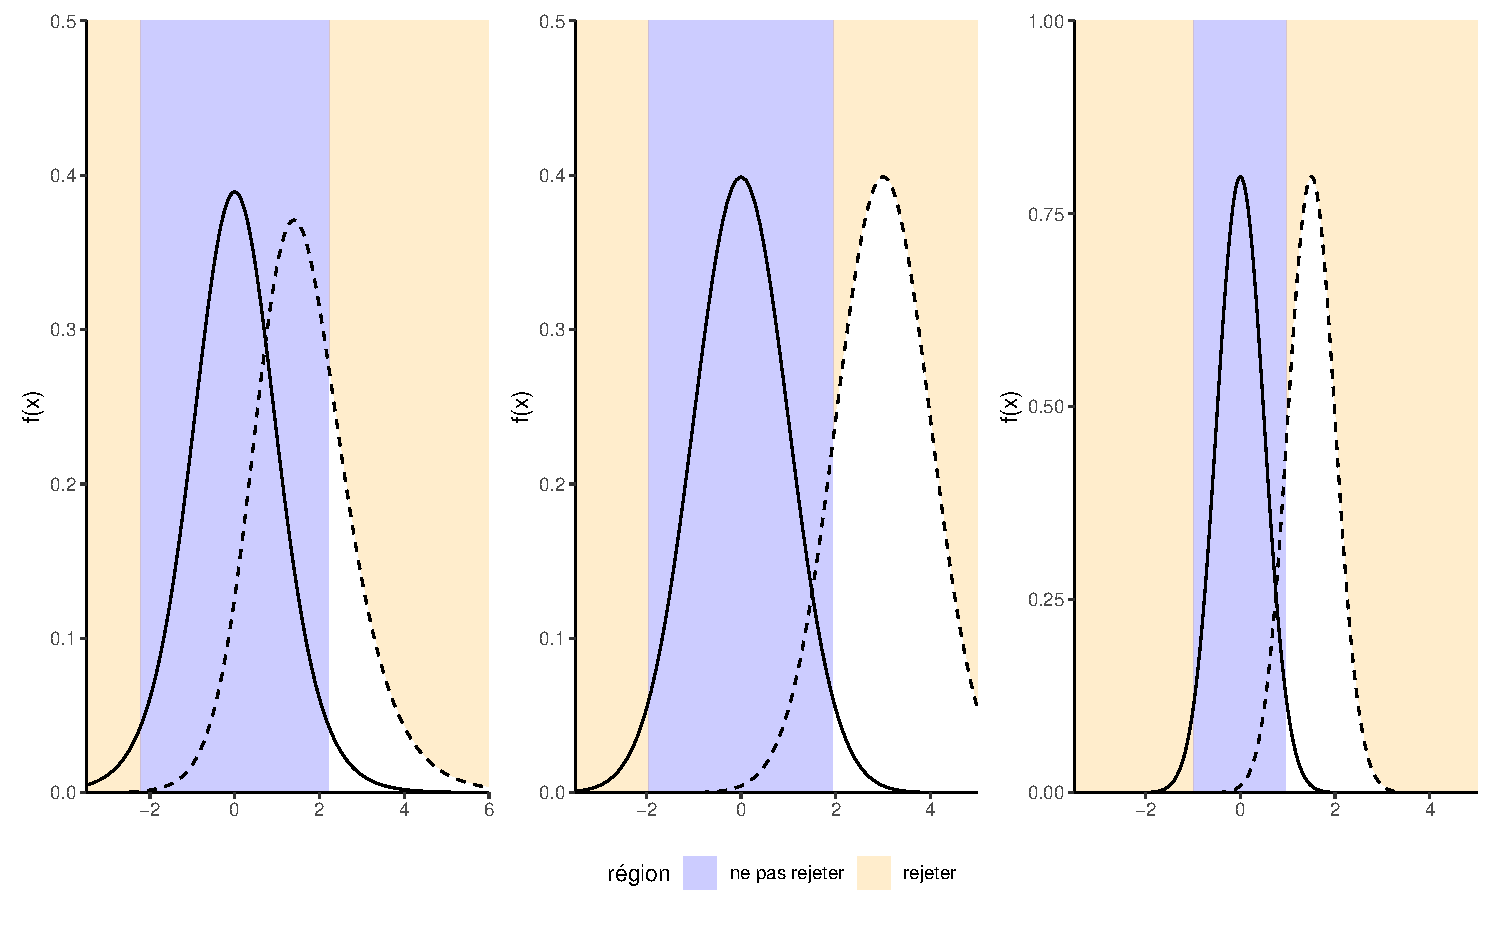
\includegraphics[width=1\textwidth,height=\textheight]{inference_files/figure-pdf/fig-puissance-1.pdf}

}

\caption{\label{fig-puissance}Comparaison de la loi nulle (ligne pleine)
et d'une alternative spécifique pour un test-\(t\) (ligne traitillée).
La puissance correspond à l'aire sous la courbe de la densité de la loi
alternative qui est dans la zone de rejet du test (en blanc). Le panneau
du milieu représente l'augmentation de la puissance suite à
l'augmentation de la taille d'effet (différence moyenne entre groupes
plus élevée) sous l'hypothèse alternative. Le panneau de droite
correspond à un scénario alternatif avec la même taille d'effet, mais
une taille d'échantillon ou une précision plus grande.}

\end{figure}%

On veut qu'un test ait une puissance élevée, c'est-à-dire, le plus près
de 1 possible. Minimalement, la puissance du test devrait être
\(\alpha\) si on rejette l'hypothèse nulle une fraction \(\alpha\) du
temps quand cette dernière est vraie. La puissance dépend de plusieurs
critères, à savoir:

\begin{itemize}
\tightlist
\item
  la taille de l'effet: plus la différence est grande entre la valeur
  postulée \(\theta_0\) du paramètre sous \(\mathscr{H}_0\) et le
  comportement observé, plus il est facile de le détecter (panneau du
  milieu de Figure~\ref{fig-puissance});
\item
  la variabilité: moins les observations sont variables, plus il est
  facile de déterminer que la différence observée est significative (les
  grandes différences sont alors moins plausibles, comme l'illustre le
  panneau de droite de Figure~\ref{fig-puissance});
\item
  la taille de l'échantillon: plus on a d'observations, plus notre
  capacité à détecter une différence significative augmente parce que
  l'erreur-type décroît avec la taille de l'échantillon à un rythme
  (ordinairement) de \(n^{-1/2}.\) La loi nulle devient aussi plus
  concentrée quand la taille de l'échantillon augmente.
\item
  le choix de la statistique de test: par exemple, les statistiques
  basées sur les rangs n'utilisent pas les valeurs numériques qu'à
  travers le rang relatif. Ces tests sont donc moins puissants parce
  qu'ils n'utilisent pas toute l'information dans l'échantillon; en
  contrepartie, ils sont souvent plus robustes en présence de valeurs
  aberrantes et si le modèle est mal spécifié. Les statistiques de test
  que nous choisirons sont souvent standards et parmi les plus
  puissantes qui soient, aussi on ne traitera pas de ce point davantage
  dans le cadre du cours.
\end{itemize}

Pour calculer la puissance d'un test, il faut choisir une alternative
spécifique. Pour des exemples simples de statistiques, on peut obtenir
une formule explicite pour la puissance. Généralement, on détermine la
puissance à l'aide de méthodes de Monte Carlo en simulant des
observations d'une alternative donnée, en calculant la statistique de
test sur le nouvel échantillon simulé et en calculant la valeur-\emph{p}
associée à notre hypothèse nulle de façon répétée. On calcule par la
suite la proportion de tests qui mènent au rejet de l'hypothèse nulle à
niveau \(\alpha,\) ce qui correspond au pourcentage de valeurs-\(p\)
inférieures à \(\alpha.\)

\section{Exemples}\label{exemples}

\begin{example}[Inégalité de genre et tests de
permutation]\protect\hypertarget{exm-rosenjerdee74}{}\label{exm-rosenjerdee74}

Nous examinons les données de Rosen et Jerdee
(\citeproc{ref-Rosen:1974}{1974}), qui étudie les stéréotypes de genre
et leur impact sur la promotion et les opportunités pour les femmes
candidates. L'expérience s'est déroulée en 1972 et les unités
expérimentales, composées de 95 superviseurs bancaires masculins, ont
reçu divers mémorandums et ont été invitées à fournir des évaluations de
candidatures pour un poste de cadre. Ils devaient prendre des décisions
sur la base des informations fournies.

Nous nous intéressons à l'expérience 1 relative à la promotion des
employés: les responsables devaient décider de promouvoir ou non un
employé au poste de directeur de succursale sur la base de
recommandations et d'évaluations du potentiel de relations avec les
clients et les employés. L'intervention des auteurs s'est concentrée sur
la description de la nature (complexité) du travail du gestionnaire
(simple ou complexe) et sur le sexe du candidat (homme ou femme): tous
les dossiers étaient par ailleurs similaires.

Pour des raisons de simplicité, nous ne considérons que le facteur sexe
et nous agrégeons sur le poste pour les \(n=93\) réponses. La table
Tableau~\ref{tbl-rosen-table1} montre le décompte des recommendations
pour chaque possibilité.

\begin{longtable}[t]{lrr}

\caption{\label{tbl-rosen-table1}Recommendations de promotion pour le
poste de gestionnaire de branche selon le sexe de la personne qui
postule.}

\tabularnewline

\toprule
 & male & female\\
\midrule
promouvoir & 32 & 19\\
ne pas promouvoir & 12 & 30\\
\bottomrule

\end{longtable}

L'hypothèse nulle qui nous intéresse ici est que le sexe n'a pas
d'impact, de sorte que la probabilité de promotion est la même pour les
hommes et les femmes. Soit \(p_{\text{h}}\) et \(p_{\text{f}}\) ces
probabilités respectives; nous pouvons donc écrire mathématiquement
l'hypothèse nulle comme \(\mathscr{H}_0: p_{\text{h}} = p_{\text{f}}\)
contre l'alternative \(\mathscr{H}_a: p_{\text{h}} \neq p_{\text{f}}\).

La statistique de test généralement employée pour les tableaux de
contingence est un test du chi carré\footnote{Si vous avez suivi des
  cours de modélisation avancés, il s'agit d'un test de score obtenu en
  ajustant une régression de Poisson avec \texttt{sexe} et
  \texttt{action} comme covariables; l'hypothèse nulle correspondant à
  l'absence de terme d'interaction entre les deux.}, qui compare les
proportions globales de promotion de chaque sous-groupe. La proportion
de l'échantillon pour les hommes est de 32/42 = \textasciitilde76\%,
contre 19/49 =\textasciitilde49\% pour les femmes. Bien que cette
différence de 16 \% semble importante, elle pourrait être trompeuse:
l'erreur type pour les proportions de l'échantillon est d'environ 3.2 \%
pour les hommes et 3.4 \% pour les femmes.

S'il n'y avait pas de discrimination fondée sur le sexe, nous nous
attendrions à ce que la proportion de personnes promues soit la même
dans l'ensemble; elle est de 51/93 ou 0.55 pour l'échantillon regroupé.
Nous pourrions nous contenter de tester la différence moyenne, mais nous
nous appuyons plutôt sur le test de contingence \(X^2_p\) de Pearson
(également appelé test du khi-carré), qui compare les chiffres attendus
(sur la base de taux de promotion égaux) aux chiffres observés,
convenablement normalisés. convenablement normalisés. Si l'écart est
important entre les chiffres attendus et les chiffres observés, cela met
en doute la véracité de l'hypothèse nulle.

Si les effectifs de chaque cellule sont importants, la distribution
nulle du test du chi-deux est bien approximée par une distribution de
\(\chi^2\). La sortie du test comprend la valeur de la statistique,
\(10.79,\) les degrés de liberté de l'approximation \(\chi^2\) et la
valeur \emph{p}, qui donne la probabilité qu'un tirage aléatoire d'une
distribution \(\chi^2_1\) soit plus grand que la statistique de test
observée \textbf{en supposant que l'hypothèse nulle est vraie}. La
valeur \emph{p} est très petite, \(0.001\), ce qui signifie qu'il est
très peu probable qu'un tel résultat soit le fruit du hasard s'il n'y a
pas eu de discrimination fondée sur le sexe.

Une autre solution pour obtenir un point de référence permettant
d'évaluer le caractère exagéré du rapport de cotes observé consiste à
utiliser des simulations: les tests de permutation sont efficaces
{[}illustrés par Jared Wilber{]}
(https://www.jwilber.me/permutationtest/). Considérons une base de
données contenant les données brutes avec 93 lignes, une pour chaque
gestionnaie, avec pour chacune un indicateur d'\texttt{action} et le
\texttt{sexe} de l'employé hypothétique présenté dans la tâche.

\begin{longtable}[t]{ll}

\caption{\label{tbl-dat-long-test-rosen-print}Les cinq premières lignes
de la base de données en format long pour l'expérience 1 de Rosen et
Jerdee (1974).}

\tabularnewline

\toprule
action & sexe\\
\midrule
promouvoir & homme\\
ne pas promouvoir & femme\\
promouvoir & homme\\
ne pas promouvoir & femme\\
ne pas promouvoir & homme\\
\bottomrule

\end{longtable}

Sous l'hypothèse nulle, le sexe n'a aucune incidence sur l'action du
gestionnaire. Cela signifie que nous pourrions dresser un portrait du
monde sans discrimination en mélangeant les étiquettes de sexe de
manière répétée. Ainsi, nous pourrions obtenir une référence en répétant
les étapes suivantes plusieurs fois :

\begin{enumerate}
\def\labelenumi{\arabic{enumi}.}
\tightlist
\item
  permuter les étiquettes pour le \texttt{sexe},
\item
  recréer un tableau de contingence en agrégeant les effectifs,
\item
  calculer une statistique de test pour le tableau simulé.
\end{enumerate}

Comme statistique de test, nous utilisons le rapport des cotes: la
probabilité d'un événement est le rapport entre le nombre de succès et
le nombre d'échecs. Dans notre exemple, il s'agirait du nombre de
dossiers promus par rapport au nombre de dossiers retenus. La
probabilité de promotion d'un homme est de \(32/12,\) alors que celle
d'une femme est de \(19/30.\) Le rapport des cotes pour un homme par
rapport à une femme est donc \(\mathsf{RC}=(32/12) / (19/30)= 4.21.\)
Sous l'hypothèse nulle, \(\mathscr{H}_0: \mathsf{OR}= 1\) (même
probabilité d'être promu) (pourquoi ?)

\begin{figure}[ht!]

\centering{

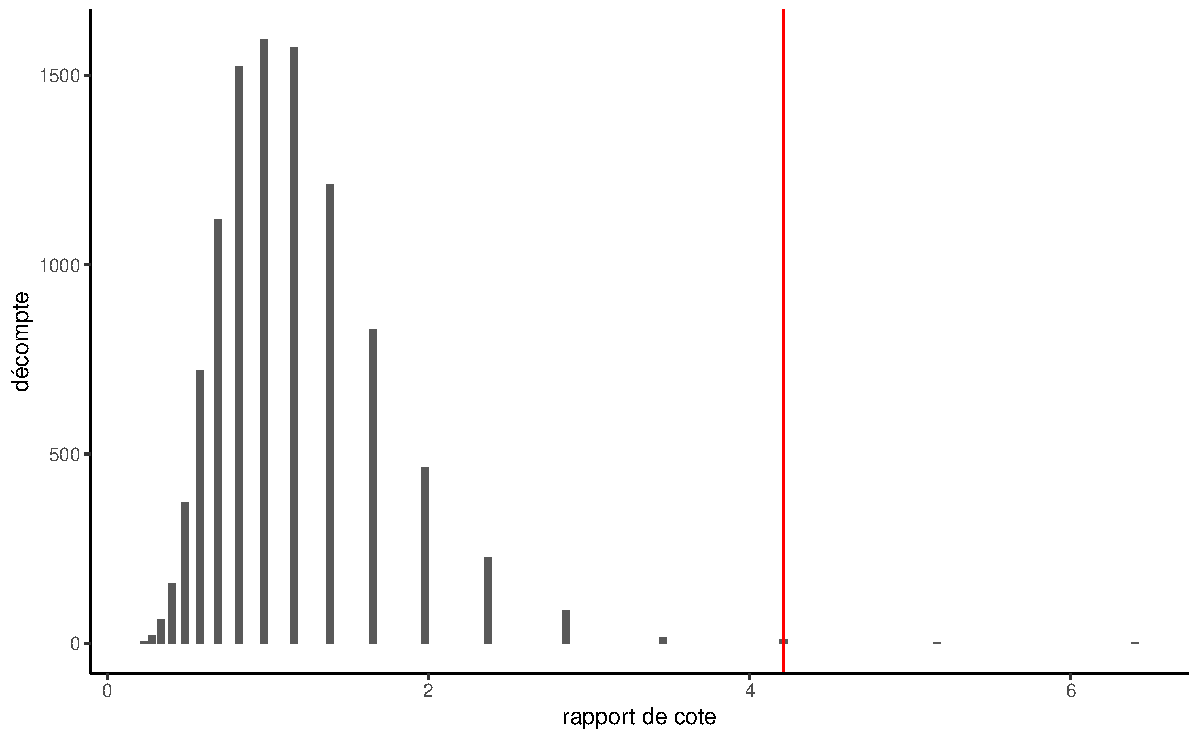
\includegraphics[width=0.85\textwidth,height=\textheight]{inference_files/figure-pdf/fig-infer-odds-ratio-permutation-1.pdf}

}

\caption{\label{fig-infer-odds-ratio-permutation}Histogramme de
simulations de la loi nulle pour le rapport de cote, obtenu par le biais
d'un test de permutation; la ligne verticale rouge indique le rapport de
cote échantillonal.}

\end{figure}%

L'histogramme de la Figure~\ref{fig-infer-odds-ratio-permutation} montre
la distribution du rapport de cotes sur la base de 10 000 permutations.
Il est rassurant de constater que nous obtenons à peu près la même
valeur \emph{p} approximative, ici 0.002.\footnote{La valeur \emph{p}
  obtenue pour le test de permutation changerait d'une exécution à
  l'autre puisque les intrants sont aléatoires. Cependant, la précision
  de la statistique est suffisante pour la prise de décision}.

L'article concluait (à la lumière de ce qui précède et d'autres
expériences)

\begin{quote}
Les résultats ont confirmé l'hypothèse selon laquelle les
administrateurs masculins ont tendance à discriminer les employées dans
les décisions concernant la promotion, le développement et la
supervision du personnel.
\end{quote}

\textbf{Récapitulatif}

\begin{itemize}
\tightlist
\item
  Paramètres du modèle: probabilité de promotion pour les hommes et les
  femmes, respectivement \(p_{\text{h}}\) et \(p_{\text{f}}\).
\item
  Hypothèses: pas de discrimination fondée sur le sexe, ce qui signifie
  une probabilité de promotion égale (hypothèse nulle
  \(\mathscr{H}_0: p_{\text{h}}=p_{\text{f}},\) contre hypothèse
  alternative \(\mathscr{H}_a: p_{\text{h}}\neq p_{\text{f}}\)).
\item
  Statistique de test: (1) test du khi-deux pour les tableaux de
  contingence et (2) rapport de cotes.
\item
  Valeur-\(p\): (1) \(.0010\) et (2) \(.0024\) pour le test de
  permutation.
\item
  Conclusion: rejeter l'hypothèse nulle, car il existe des preuves d'une
  discrimination fondée sur le sexe, avec une probabilité de promotion
  différente pour les hommes et les femmes.
\end{itemize}

Conformément aux directives de l'APA, la statistique \(\chi^2\) serait
présentée sous la forme \(\chi^2(1, n = 93) = 10.79\), \(p = .001\) en
même temps que les effectifs et les proportions de l'échantillon.

\end{example}

\begin{example}[L'élément de surprise d'une prise de contact
inattendue]\protect\hypertarget{exm-LiuRimMinMin2023E1}{}\label{exm-LiuRimMinMin2023E1}

Liu et al. (\citeproc{ref-Liu.Rim.Min.Min:2023}{2023}) étudie les
interactions sociales et l'impact de la surprise sur les personnes qui
contactent de vieilles connaissances de manière inattendue. L'expérience
1 se concentre sur des questionnaires où la condition expérimentale est
l'appréciation perçue du fait d'envoyer une communication à quelqu'un
avec qui on n'a pas correspondu depuis longtemps (par opposition au fait
de se faire contacter). L'étude a utilisé un questionnaire envoyé à 200
adultes américains recrutés sur la plateforme Prolific Academic.
L'indice de réponse consiste en la moyenne de quatre questions mesurées
sur une échelle de Likert allant de 1 à 7, les valeurs les plus élevées
indiquant une plus grande appréciation de la prise de contact.

Nous pouvons commencer par examiner les statistiques sommaires des
variables sociodémographiques (sexe et âge) afin d'évaluer si
l'échantillon est représentatif de la population générale dans son
ensemble. La proportion d'« autres » (comprenant les personnes non
binaires) est beaucoup plus élevée que celle du recensement général, et
la population est plutôt jeune selon
Tableau~\ref{tbl-LRMMS1-summarystat-a}.

\begin{longtable}[t]{lrrrr}

\caption{\label{tbl-LRMMS1-summarystat-a}Statistiques descriptives de
l'âge des participants, et décompte par genre.}

\tabularnewline

\toprule
genre & min & max & moyenne & n\\
\midrule
homme & 18 & 78 & 32.0 & 105\\
femme & 19 & 68 & 36.5 & 92\\
autre & 24 & 30 & 27.7 & 3\\
\bottomrule

\end{longtable}

\begin{longtable}[t]{lrrr}

\caption{\label{tbl-LRMMS1-summarystat-b}Appréciation moyenne
(écart-type), et nombre de participants par condition expérimentale.}

\tabularnewline

\toprule
rôle & moyenne & écart-type & n\\
\midrule
initiateur & 5.50 & 1.28 & 103\\
destinataire & 5.87 & 1.27 & 97\\
\bottomrule

\end{longtable}

Comme il n'y a que deux groupes sans chevauchements (c'est à dire que
les personnes ont un seul rôle), soit initiateur ou destinataire, le
test logique à utiliser est un test-\(t\) pour deux échantillons
indépendants, ou une variante de celui-ci. En utilisant la statistique
du \(t\)-test de Welch, la moyenne et l'écart-type de chaque groupe sont
estimés à l'aide des données fournies.

Le logiciel renvoie comme valeur du test , ce qui conduit au rejet de
l'hypothèse nulle d'absence de différence d'appréciation en fonction du
rôle de l'individu (initiateur ou destinataire). La différence moyenne
estimée est \(\Delta M = -0.37\), 95\% CI \([-0.73, -0.01]\); puisque
\(0\) n'est pas inclus dans l'intervalle de confiance, nous rejetons
également l'hypothèse nulle au niveau 5\%. L'estimation suggère que les
initiateurs sous-estiment l'importance de contacter de manière
inattendue.\footnote{En supposant que la variance de chaque sous-groupe
  soit égale, nous aurions pu utiliser un \(t\)-test à deux échantillons
  à la place. La différence dans la conclusion est insignifiante, avec
  une valeur \emph{p} presque égale}.

\textbf{Récapitulatif}

\begin{itemize}
\tightlist
\item
  Paramètres du modèle: score d'appréciation moyen \(\mu_{\mathrm{i}}\)
  et \(\mu_{\mathrm{d}}\) des initiateurs et des destinataires,
  respectivement.
\item
  Hypothèse: le score d'appréciation attendu est le même pour les
  initiateurs et les destinataires,
  \(\mathscr{H}_0: \mu_{\mathrm{i}}=\mu_{\mathrm{d}}\) contre
  l'alternative
  \(\mathscr{H}_0: \mu_{\mathrm{i}} \neq \mu_{\mathrm{r}}\) qu'ils sont
  différents.
\item
  Statistique de test: test-\(t\) de Welch pour deux échantillons
  indépendants
\item
  Valeur-\(p\): 0.041
\item
  Conclusion: rejet de l'hypothèse nulle, le score moyen d'appréciation
  diffère selon le rôle tenu.
\end{itemize}

\end{example}

\begin{example}[Les communications virtuelles réduisent le nombre
d'idées
créatives]\protect\hypertarget{exm-BrucksLevav22}{}\label{exm-BrucksLevav22}

Une étude de Nature a réalisé une expérience pour voir comment les
communications virtuelles impactent le travail d'équipe en comparant le
nombre d'idées créatives générées par des binômes au cours d'une tempête
d'idée, ainsi que leur qualité telle que mesurée par des arbitres
externes. L'échantillon était composé de 301 paires de participants qui
ont interagi par vidéoconférence ou en face à face.

Les auteurs ont comparé le nombre d'idées créatives, un sous-ensemble
d'idées générées avec un score de créativité supérieur à la moyenne. Le
nombre moyen d'idées créatives pour le face à face est \(7.92\) idées
(écart-type \(3.40\)), comparativement à \(6.73\) idées (écart-type¸
\(3.27\)) pour la vidéoconférence.

Brucks et Levav (\citeproc{ref-Brucks.Levav:2022}{2022}) a utilisé un
modèle de régression binomiale négative: dans leur modèle, le nombre
moyen d'idées créatives générées est \begin{align*}
\mathsf{E}(\texttt{ncreative}) = \exp(\beta_0 + \beta_1 \texttt{video})
\end{align*} où \(\texttt{video}=0\) si la paire se trouve dans la même
pièce et \(\texttt{video}=1\) si elle interagit plutôt par
vidéoconférence.

Le nombre moyen d'idées pour la vidéoconférence est donc
\(\exp(\beta_1)\) multiplié par celui du face à face: l'estimation du
facteur multiplicatif est \(\exp(\beta_1)\) est \(0.85\) 95\% CI
\([0.77, 0.94]\).

L'absence de différence entre les conditions expérimentales se traduit
par l'hypothèse nulle \(\mathscr{H}_0: \beta_1=0\) vs
\(\mathscr{H}_0: \beta_1 \neq 0\) ou, de manière équivalente,
\(\mathscr{H}_0: \exp(\beta_1)=1\). Le test du rapport de vraisemblance
comparant le modèle de régression avec et sans \(\texttt{video}\) la
statistique est \(R=9.89\) (valeur-\(p\) basée sur \(\chi^2_1\) de
\(.002\)). Nous concluons que le nombre moyen d'idées est différent, les
statistiques sommaires suggérant que les paires virtuelles génèrent
moins d'idées.

Si nous avions eu recours à un test-\(t\) pour deux échantillons
indépendants, nous aurions trouvé une différence moyenne dans le nombre
d'idées créatives de \(\Delta M = 1.19\), 95\% CI \([0.43, 1.95]\),
\(t(299) = 3.09\), \(p = .002\).

Les deux tests reposent sur des hypothèses légèrement différentes, mais
aboutissent à des conclusions similaires: il a de forts indices que le
nombre d'idées créatives est plus faible lorsque les personnes
interagissent par vidéoconférence.

\end{example}

\begin{example}[Prix de billets de trains à grande vitesse
espagnols]\protect\hypertarget{exm-prix-trains-tests}{}\label{exm-prix-trains-tests}

La compagnie nationale de chemin de fer
\href{https://www.renfe.com/}{Renfe} gère les trains régionaux et les
trains à haute vitesse dans toute l'Espagne. Les prix des billets vendus
par Renfe sont
\href{https://www.kaggle.com/thegurusteam/spanish-high-speed-rail-system-ticket-pricing}{aggrégés}
par une compagnie. On s'intéresse ici à une seule ligne,
Madrid--Barcelone. Notre question scientifique est la suivante: est-ce
que le prix des billets pour un aller (une direction) est plus chère
pour un retour? Pour ce faire, on considère un échantillon de 10000
billets entre les deux plus grandes villes espagnoles. On s'intéresse au
billets de TGV vendus (AVE) au tarif Promotionnel. Notre statistique de
test sera simplement la différence de moyenne entre les deux
échantillons: la différence entre le prix en euros d'un train
Madrid--Barcelone (\(\mu_1\)) et le prix d'un billet Barcelone--Madrid
(\(\mu_2\)) est \(\mu_1-\mu_2\) et notre hypothèse nulle est qu'il n'y a
aucune différence de prix, soit \(\mathscr{H}_0: \mu_1-\mu_2=0.\)

On utilise de nouveau le test de Welch pour deux échantillons en
filtrant les données pour ne conserver que les billets au tarif Promo:
la moyenne des billets Barcelone-Madrid est 82.11 euros, ceux pour
Madrid-Barcelone 82.56 euros et la valeur de la statistique de Welch est
-1.33. Si on utilise l'approximation normale, on obtient une
valeur-\(p\) de 0.18.

Plutôt que d'utiliser la loi asymptotique (qui est valide pour de grands
échantillons à cause du théorème central limite), on peut considérer une
approximation sous une hypothèse moins restrictive en supposant que les
données sont échangeables. Sous l'hypothèse nulle, il n'y aucune
différence entre les deux destinations et les étiquettes pour la
destination (une variable catégorielle binaire) sont arbitraires. On
pourrait considérer les mêmes données, mais avec une permutation des
variables explicatives: c'est ce qu'on appelle un
\href{https://www.jwilber.me/permutationtest/}{test de permutation}. On
va recréer deux groupes de taille identique à notre échantillon
original, mais en changeant les observations. On recalcule la
statistique de test sur ces nouvelle données (si on a une poignée
d'observations, il est possible de lister toutes les permutations
possibles; typiquement, il suffit de considérer un grand nombre de
telles permutations, disons 9999). Pour chaque nouveau jeu de données,
on calculera la statistique de test et on calculera le rang de notre
statistique par rapport à cette référence. Si la valeur de notre
statistique observée sur l'échantillon original est extrême en
comparaison, c'est autant de preuves contre l'hypothèse nulle.

\begin{figure}[ht!]

\centering{

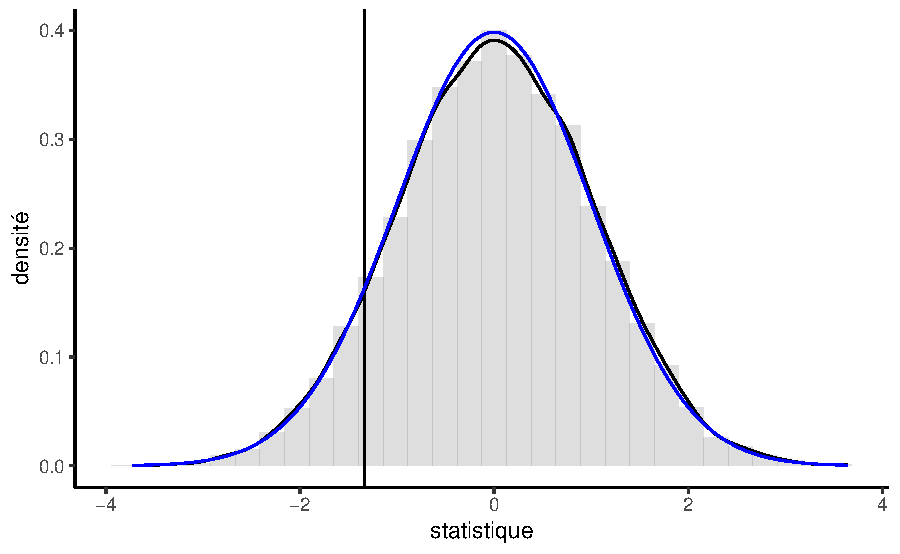
\includegraphics[width=0.85\textwidth,height=\textheight]{inference_files/figure-pdf/fig-renfepermut-1.pdf}

}

\caption{\label{fig-renfepermut}Approximation par permutation de la loi
nulle de la statistique de test de Welch (histogramme et trait noir) et
loi asymptotique normale standard (trait bleu) pour le prix de billets
de trains AVE au tarif promotionnel entre Madrid et Barcelone. La valeur
de la statistique de test de l'échantillon original est représentée par
un trait vertical.}

\end{figure}%

La valeur-\emph{p} du test de permutation, \(0.186,\) est la proportion
de statistiques plus extrêmes que celle observée. Cette valeur-\emph{p}
est quasi-identique à celle de l'approximation de Satterthwaite, à
savoir \(0.182\) (la loi Student-\(t\) est numériquement équivalente à
une loi standard normale avec autant de degrés de liberté), tel que
représenté dans la Figure~\ref{fig-renfepermut}. Malgré que notre
échantillon soit très grand, avec \(n=8059\) observations, la différence
n'est pas jugée significative. Avec un échantillon de deux millions de
billets, on pourrait estimer précisément la moyenne (au centime près):
la différence de prix entre les deux destinations et cette dernière
deviendrait statistiquement significative. Elle n'est pas en revanche
pas pertinente en partique, car une différence de \(0.28\) euros sur un
prix moyen de \(82.56\) euros est quantité négligeable.

\end{example}

\bookmarksetup{startatroot}

\chapter*{Bibliographie}\label{bibliographie}
\addcontentsline{toc}{chapter}{Bibliographie}

\markboth{Bibliographie}{Bibliographie}

\phantomsection\label{refs}
\begin{CSLReferences}{1}{0}
\bibitem[\citeproctext]{ref-Brodeur:2021}
Brodeur, Mathieu, Perrine Ruer, Pierre-Majorique Léger, et Sylvain
Sénécal. 2021. {«~Smartwatches are more distracting than mobile phones
while driving: Results from an experimental study~»}. \emph{Accident
Analysis \& Prevention} 149: 105846.
\url{https://doi.org/10.1016/j.aap.2020.105846}.

\bibitem[\citeproctext]{ref-Brucks.Levav:2022}
Brucks, Melanie S., et Jonathan Levav. 2022. {«~Virtual communication
curbs creative idea generation~»}. \emph{Nature} 605 (7908): 108‑12.
\url{https://doi.org/10.1038/s41586-022-04643-y}.

\bibitem[\citeproctext]{ref-Duke.Amir:2023}
Duke, Kristen E., et On Amir. 2023. {«~The Importance of Selling
Formats: When Integrating Purchase and Quantity Decisions Increases
Sales~»}. \emph{Marketing Science} 42 (1): 87‑109.
\url{https://doi.org/10.1287/mksc.2022.1364}.

\bibitem[\citeproctext]{ref-Lee.Choi:2019}
Lee, Kiljae, et Jungsil Choi. 2019. {«~Image-text inconsistency effect
on product evaluation in online retailing~»}. \emph{Journal of Retailing
and Consumer Services} 49: 279‑88.
\url{https://doi.org/10.1016/j.jretconser.2019.03.015}.

\bibitem[\citeproctext]{ref-Liu.Rim.Min.Min:2023}
Liu, Peggy J., SoYon Rim, Lauren Min, et Kate E. Min. 2023. {«~The
surprise of reaching out: Appreciated more than we think.~»}
\emph{Journal of Personality and Social Psychology} 124 (4): 754‑71.
\url{https://doi.org/10.1037/pspi0000402}.

\bibitem[\citeproctext]{ref-McCullagh.Nelder:1989}
McCullagh, P., et J. A. Nelder. 1989. \emph{Generalized linear models}.
{S}econd edition. London: Chapman \& Hall.

\bibitem[\citeproctext]{ref-Moon.VanEpps:2023}
Moon, Alice, et Eric M VanEpps. 2023. {«~Giving Suggestions: Using
Quantity Requests to Increase Donations~»}. \emph{Journal of Consumer
Research} 50 (1): 190‑210. \url{https://doi.org/10.1093/jcr/ucac047}.

\bibitem[\citeproctext]{ref-Rosen:1974}
Rosen, B., et T. H. Jerdee. 1974. {«~Influence of sex role stereotypes
on personnel decisions.~»} \emph{Journal of Applied Psychology} 59:
9‑14.

\bibitem[\citeproctext]{ref-Sokolova:2023}
Sokolova, Tatiana, Aradhna Krishna, et Tim Döring. 2023. {«~Paper Meets
Plastic: The Perceived Environmental Friendliness of Product
Packaging~»}. \emph{Journal of Consumer Research} 50 (3): 468‑91.
\url{https://doi.org/10.1093/jcr/ucad008}.

\end{CSLReferences}


\backmatter


\end{document}
